\documentclass[11pt]{article}

\usepackage[left=1.25in,top=1.25in,right=1.25in,bottom=1.25in,head=1.25in]{geometry}
\usepackage{amsfonts,amsmath,amssymb,amsthm}

\title{Summary and discussion of: ``Matrix Completion and Low-Rank SVD via
	Fast Alternating Least Squares''\\
%% replace wih paper title 
\large{MATH5472 report} }
		\author{Chengyu TAO}
%% replace with your names
\date{2021-12-10}
\usepackage[colorlinks,
linkcolor=blue,
anchorcolor=blue,
citecolor=blue]{hyperref}
\usepackage{float}
\usepackage{natbib}
\usepackage{algorithm}
\usepackage{amsmath}
\usepackage{graphicx}
\usepackage{enumerate}
\usepackage{caption}
\usepackage{multirow}
\usepackage{nicefrac}
\usepackage{mathabx}
\usepackage{subfigure}
\usepackage{amssymb}
\usepackage{algorithm}
\usepackage[title]{appendix}
\usepackage{algpseudocode}
\begin{document}
\maketitle
\section{Introduction}
In this report, we will summarize \cite{hastie2015matrix}'s paper about matrix completion problem. The proposed method is named as \textbf{softImpute-ALS}. The main characteristic of \textbf{softImpute-ALS} is its fast computation speed compared with the two popular methods  \textbf{softImpute} \citep{mazumder2010spectral} and \textbf{ MMMF}(maximum-margin matrix factorization) \citep{srebro2004maximum}. In fact, \textbf{softImpute-ALS} borrows ideas from \textbf{softImpute} and \textbf{ MMMF}. It combines the two methods to achieve relatively lower time complexity. We will briefly summary \textbf{softImpute} and \textbf{MMMF} firstly.

\textbf{softImpute} solves the following problem
\begin{equation}
\underset{\boldsymbol{M}}{\operatorname{min}} \ \ F(\boldsymbol{M}):=\frac{1}{2}\left\|P_{\Omega}(\boldsymbol{X}-\boldsymbol{M})\right\|_{F}^{2}+\lambda\|\boldsymbol{M}\|_{*},
\label{eq:nuclear form}
\end{equation}
where $P_{\Omega}(\cdot)$ is a projector onto $\Omega$ and $\Omega$ is the positions of known entries of $\boldsymbol{X}$. Considering a Majority-Minimization (MM) framework, a surrogate function $Q(\boldsymbol{M}| \tilde{\boldsymbol{M}})=\frac{1}{2}\left\|P_{\Omega}(\boldsymbol{X})+P_{\Omega}^{\perp}(\tilde{\boldsymbol{M}})-\boldsymbol{M}\right\|_{F}^{2}+\lambda\|\boldsymbol{M}\|_{*}$ can be constructed such that $Q(\tilde{\boldsymbol{M}}|\tilde{\boldsymbol{M}})=F(\tilde{\boldsymbol{M}})$ and $Q(\boldsymbol{M}|\tilde{\boldsymbol{M}})\geq F(\boldsymbol{M})$. The second property can be derived using the identity $\boldsymbol{M}=P_{\Omega}(\boldsymbol{M})+P_{\Omega}^{\perp}(\boldsymbol{M})$. Note that, \cite{mazumder2010spectral} did not explicitly interpret it by the MM framework. However, the \textbf{Lemma 2} \citep{mazumder2010spectral} is indeed consistent with the MM method.  

Therefore, the  problem (\ref{eq:nuclear form}) can be replaced by solving the following problem iteratively
\begin{equation}
\boldsymbol{M}^{k+1} =\underset{\boldsymbol{M}}{\operatorname{argmin}} \ \ Q(\boldsymbol{M}|\boldsymbol{M}^k)=\frac{1}{2}\left\|P_{\Omega}(\boldsymbol{X})+P_{\Omega}^{\perp}(\boldsymbol{M}^k)-\boldsymbol{M}\right\|_{F}^{2}+\lambda\|\boldsymbol{M}\|_{*}.
\label{eq:softimpute}
\end{equation}

The above problem has closed-form solution based on singular value decomposition (SVD). Denote $\boldsymbol{X}^*=P_{\Omega}(\boldsymbol{X})+P_{\Omega}^{\perp}(\boldsymbol{M}^k)$ and  $X^*=UDV^T$ as its SVD, then, $\boldsymbol{M}^{k+1}=U\mathcal{S}_{\lambda}(D)V^T$, where $\mathcal{S}_{\lambda}(D)$ operates on each entry $D_{i,i}$ such that $\mathcal{S}_{\lambda}(D)_{i,i} = \max (D_{i,i}-\lambda,0)$ and 0 elsewhere. 

The main limitation of \textbf{softImpute} is the high time complexity of SVD when $\boldsymbol{X}^*$ has very large dimension. Generally, if $\boldsymbol{X}^* \in R^{m\times n}$, the time complexity of SVD of $\boldsymbol{X}^*$ is $O(mn \min(m,n))$. Though the special structure of $\boldsymbol{X}^*$ and warm start of SVD can be explored, the computational load in high-dimension cases is still burdensome.

\textbf{ MMMF} is an alternative method. Using the following inequality 
\begin{equation}
	\|\boldsymbol{M}\|_{*}=\min _{\boldsymbol{A}, \boldsymbol{B}: \boldsymbol{M}=\boldsymbol{A} \boldsymbol{B}^{T}} \frac{1}{2}\left(\|\boldsymbol{A}\|_{F}^{2}+\|\boldsymbol{B}\|_{F}^{2}\right).
	\label{eq:mmmf}
\end{equation}
\cite{srebro2004maximum}'s goal is to solve the following problem
\begin{equation}
	\underset{\boldsymbol{A},\boldsymbol{B}}{\operatorname{min}} \ \ G(\boldsymbol{A},\boldsymbol{B}):=\frac{1}{2}\left\|P_{\Omega}(\boldsymbol{X}-\boldsymbol{AB}^T)\right\|_{F}^{2}+\frac{\lambda}{2}\left(\|\boldsymbol{A}\|_{F}^{2}+\|\boldsymbol{B}\|_{F}^{2}\right),
	\label{eq:mmmf_als}
\end{equation}
	where $\boldsymbol{M} \in R^{m \times n }$, $\boldsymbol{A} \in R^{m \times r }$, and $\boldsymbol{B} \in R^{n \times r }$. The two problems (\ref{eq:mmmf}) and (\ref{eq:nuclear form}) produce equivalent results under certain conditions, due to the space limitation, for more details, we refer to the raw paper \citep{hastie2015matrix}. This problem is biconvex and can be solved by alternating least square method. When $\boldsymbol{A}$ is fixed, the optimization of $\boldsymbol{B}$ consists of a series of  subproblems ($r$ times) that each row of $\boldsymbol{B}$ can be obtained by an independent vector ridge regression. Symmetrically, optimizing $\boldsymbol{B}$ follows the same procedure. The independence is caused by the projector $P_{\Omega}(\cdot)$ that for each column the locations of known row entries are different such that the regression matrices are different. 

The independence of vector ridge regressions will bring relatively higher computational complexity with $r$ times larger than that of only one matrix ridge regression with an unchanged regression matrix. On the other side,  
if we factorize $\boldsymbol{M} = \boldsymbol{AB}^T$ in Eq. (\ref{eq:softimpute}) and use Eq. (\ref{eq:mmmf}), we can solve the following problem in the framework of  \textbf{softImpute} iteratively
\begin{equation}
	\begin{split}
	\boldsymbol{A}^{k+1},\boldsymbol{B}^{k+1} =&\underset{\boldsymbol{A},\boldsymbol{B}}{\operatorname{argmin}} \ \ L(\boldsymbol{A},\boldsymbol{B})=\\ &\frac{1}{2}\left\|P_{\Omega}(\boldsymbol{X})+P_{\Omega}^{\perp}(\boldsymbol{A}^k(\boldsymbol{B}^k)^T)-\boldsymbol{AB}^T\right\|_{F}^{2}+\frac{\lambda}{2}\left(\|\boldsymbol{A}\|_{F}^{2}+\|\boldsymbol{B}\|_{F}^{2}\right).
	\label{eq:softimpute_als}
	\end{split}
\end{equation}

We can find that the above problem (\ref{eq:softimpute_als}) has the same form as the problem (\ref{eq:mmmf_als}). Interestingly, $P_{\Omega}(\boldsymbol{X})+P_{\Omega}^{\perp}(\boldsymbol{A}^k(\boldsymbol{B}^k)^T)$ do not contain any missing entries, which implies that using  alternating least square method to solve (\ref{eq:softimpute_als}) only requires matrix ridge regressions. From this perspective, it shows potential faster computation speed than that of \textbf{ MMMF}. Moreover,  SVD is also unnecessary in the above problem (\ref{eq:softimpute_als}), thus, it is also expected to be better than \textbf{softImpute} in terms of time complexity. This problem (\ref{eq:softimpute_als}) is the central step of \textbf{softImpute-ALS}. Next, we will show more details about \textbf{softImpute-ALS}.


\section{Summary of softImpute-ALS}

	We will present the main procedure of \textbf{softImpute-ALS} at first, which is followed by some further comments. 
	
\textbf{SoftImpute-ALS} is concluded in Algorithm \ref{alg_1}. Actually,  $\boldsymbol{A}$ and $\boldsymbol{B}$ are orthogonal factorized by $\boldsymbol{U}\boldsymbol{D}$ and $\boldsymbol{V}\boldsymbol{D}$ respectively. Then, when using  alternating least square method to solve the problem (\ref{eq:softimpute_als}), it consists of two matrix ridge regressions as shown in Algorithm \ref{alg_1}. In each iteration, we have the following relationship
\begin{equation}
	\begin{split}
	W(\bar{\boldsymbol{A}},\bar{\boldsymbol{B}})\leq L(\boldsymbol{A}^k,\tilde{\boldsymbol{B}}) \leq L(\boldsymbol{A}^k,\boldsymbol{B}^k)=W(\boldsymbol{A}^k,\boldsymbol{B}^k) \\
	W(\boldsymbol{A}^{k+1},\boldsymbol{B}^{k+1})\leq	L(\tilde{\boldsymbol{A}},\bar{\boldsymbol{B}})\leq L(\bar{\boldsymbol{A}},\bar{\boldsymbol{B}}) =W(\bar{\boldsymbol{A}},\bar{\boldsymbol{B}}),
	\end{split}
\end{equation}
where $W(\boldsymbol{A},\boldsymbol{B}) =\frac{1}{2}\left\|P_{\Omega}(\boldsymbol{X})+P_{\Omega}^{\perp}(\boldsymbol{A}^k(\boldsymbol{B}^k)^T)-\boldsymbol{AB}^T\right\|_{F}^{2}+\frac{\lambda}{2}\|\boldsymbol{AB}^T\|_{*} $. The proof relies on Eq. (\ref{eq:mmmf}), we do not give detailed proof here. Therefore, the orthogonal factorization \footnote{In fact, the purpose of the above orthogonal factorization is not very clear. \cite{panagoda2021convergence} claim that it will produce faster convergence rate if $P_{\Omega}(\boldsymbol{X})+P_{\Omega}^{\perp}(\boldsymbol{A}^k(\boldsymbol{B}^k)^T)$ is low rank, however, it is a kind of structure \textit{sparse plus low rank}.} can be regarded as modifying the problem (\ref{eq:softimpute_als}) that it directly deals with the following problem
\begin{equation}
	\begin{split}
		\boldsymbol{A}^{k+1},\boldsymbol{B}^{k+1} =&\underset{\boldsymbol{A},\boldsymbol{B}}{\operatorname{argmin}} \ \ W(\boldsymbol{A},\boldsymbol{B})=\\ &\frac{1}{2}\left\|P_{\Omega}(\boldsymbol{X})+P_{\Omega}^{\perp}(\boldsymbol{A}^k(\boldsymbol{B}^k)^T)-\boldsymbol{AB}^T\right\|_{F}^{2}+\frac{\lambda}{2}\|\boldsymbol{AB}^T\|_{*}.
		\label{eq:softimpute_als_orth}
	\end{split}
\end{equation}
	
	\begin{algorithm}[h]
	\caption{\small \textbf{softImpute-ALS}}
	\label{alg_1}
	\textbf{Input:} matrix $\boldsymbol{X}$, stop threshold $\epsilon$\\
	\textbf{Initialize:} $\boldsymbol{A}=\boldsymbol{U}\boldsymbol{D}$, where $\boldsymbol{U}\in R^{m \times r }$ is random orthogonal matrix and $\boldsymbol{D} = \boldsymbol{I}_r$. $\boldsymbol{B}=\boldsymbol{V}\boldsymbol{D}$, where $\boldsymbol{V}=\boldsymbol{0}$. Note that, any warm start can be used for initialization. \\
	\textbf{Output:} $\boldsymbol{A}$,$\boldsymbol{B}$,$\boldsymbol{U}$,$\boldsymbol{D}$,$\boldsymbol{V}$.
	\begin{algorithmic}
		\Repeat
		\State Set $\boldsymbol{A}_{old}=\boldsymbol{A}$ and $\boldsymbol{B}_{old}=\boldsymbol{B}$.
		\State Set $\boldsymbol{X}^*=P_{\Omega}(\boldsymbol{X})+P_{\Omega}^{\perp}(\boldsymbol{A}\boldsymbol{B}^T)$, and then calculate $\tilde{\boldsymbol{B}}^T=(\boldsymbol{D}^2+\lambda\boldsymbol{I}_r)^{-1}\boldsymbol{D}\boldsymbol{U}^T\boldsymbol{X}^*$. Find the SVD $\tilde{\boldsymbol{B}}\boldsymbol{D} = \tilde{\boldsymbol{U}}\tilde{\boldsymbol{D}}^2\tilde{\boldsymbol{V}}^T$. 
		\State Update $\boldsymbol{V} \leftarrow \tilde{\boldsymbol{U}}$, $\boldsymbol{D} \leftarrow \tilde{\boldsymbol{D}}$, $\boldsymbol{U} \leftarrow \boldsymbol{U}\tilde{\boldsymbol{V}}$, $\bar{\boldsymbol{A}} \leftarrow \boldsymbol{U}\boldsymbol{D}$, and $\bar{\boldsymbol{B}} \leftarrow \boldsymbol{V}\boldsymbol{D}$.
		\State Set $\boldsymbol{X}^*=P_{\Omega}(\boldsymbol{X})+P_{\Omega}^{\perp}(\bar{\boldsymbol{A}}\bar{\boldsymbol{B}}^T)$, and then calculate $\tilde{\boldsymbol{A}}^T=(\boldsymbol{D}^2+\lambda\boldsymbol{I}_r)^{-1}\boldsymbol{D}\boldsymbol{V}^T(\boldsymbol{X}^*)^T$. Find the SVD $\tilde{\boldsymbol{A}}\boldsymbol{D} = \tilde{\boldsymbol{U}}\tilde{\boldsymbol{D}}^2\tilde{\boldsymbol{V}}^T$. 
		\State Update $\boldsymbol{U} \leftarrow \tilde{\boldsymbol{U}}$, $\boldsymbol{D} \leftarrow \tilde{\boldsymbol{D}}$, $\boldsymbol{V} \leftarrow \boldsymbol{V}\tilde{\boldsymbol{V}}$, $\boldsymbol{A} \leftarrow \boldsymbol{U}\boldsymbol{D}$, and $\boldsymbol{B} \leftarrow \boldsymbol{V}\boldsymbol{D}$.
		
		\Until{$\dfrac{\left\|\boldsymbol{A}\boldsymbol{B}^T-\boldsymbol{A}_{old}\boldsymbol{B}_{old}^T\right\|_F^2}{\left\|\boldsymbol{A}_{old}\boldsymbol{B}_{old}^T\right\|_F^2} \leq \epsilon$}
	\end{algorithmic}
\end{algorithm}

Similarly, we provide the non-orthogonal version of \textbf{softImpute-ALS}, we name it as \textbf{softImpute-ALS-NSBS}(non-subspace iteration). This algorithm is illustrated in Algorithm \ref{alg_2}.

	\begin{algorithm}[h]
	\caption{\small \textbf{softImpute-ALS-NSBS}}
	\label{alg_2}
	\textbf{Input:} matrix $\boldsymbol{X}$, stop threshold $\epsilon$\\
	\textbf{Initialize:} $\boldsymbol{A}=\boldsymbol{A}_0$ and $\boldsymbol{B}=\boldsymbol{0}$. Note that, any warm start can be used for initialization.\\
	\textbf{Output:} $\boldsymbol{A}$,$\boldsymbol{B}$
	\begin{algorithmic}
		\Repeat
		\State Set $\boldsymbol{A}_{old}=\boldsymbol{A}$ and $\boldsymbol{B}_{old}=\boldsymbol{B}$.
		\State Set $\boldsymbol{X}^*=P_{\Omega}(\boldsymbol{X})+P_{\Omega}^{\perp}(\boldsymbol{A}\boldsymbol{B}^T)$, and then update $\boldsymbol{B}\leftarrow (\boldsymbol{X}^*)^T\boldsymbol{A}(\boldsymbol{D}^2+\lambda\boldsymbol{I}_r)^{-1}$.
		\State Set $\boldsymbol{X}^*=P_{\Omega}(\boldsymbol{X})+P_{\Omega}^{\perp}(\boldsymbol{A}\boldsymbol{B}^T)$, and then update $\boldsymbol{A}\leftarrow (\boldsymbol{X}^*)\boldsymbol{B}(\boldsymbol{D}^2+\lambda\boldsymbol{I}_r)^{-1}$.

		\Until{$\dfrac{\left\|\boldsymbol{A}\boldsymbol{B}^T-\boldsymbol{A}_{old}\boldsymbol{B}_{old}^T\right\|_F^2}{\left\|\boldsymbol{A}_{old}\boldsymbol{B}_{old}^T\right\|_F^2} \leq \epsilon$}
	\end{algorithmic}
\end{algorithm}

Another benefit from orthogonal factorization is that the output of \textbf{softImpute-ALS} can be used as warm start for \textbf{softImpute}, while \textbf{softImpute-ALS-NSBS} needs an additional SVD to refactorize. For large-scale problem, the refactorization is time-consuming. In addition, we should note that \textbf{softImpute-ALS} add a rank-r constraint, which plays a trade-off between accuracy and efficiency. 

\textbf{SoftImpute-ALS} converges at the rate $O(\dfrac{1}{K})$. For detailed theoretic analysis of the convergence behavior of \textbf{SoftImpute-ALS}, one can refer the raw paper \citep{hastie2015matrix}. We are more concerned about the time-complexity. 
The total costs of an iteration of \textbf{SoftImpute-ALS} and \textbf{SoftImpute-ALS-NSBS}  are $O(2r|\Omega| + mr^2 +3nr^2 + r^3)$. The cost of a rank-$r^{\prime}$ SVD of \textbf{softImpute} with current rank $\tilde{r}$ is $O(r^{\prime}|\Omega| + mr^{\prime}\tilde{r} +nr^{\prime}\tilde{r})$. At the first several steps, $r^{\prime}$ and $\tilde{r}$ are very large and there is no good warm start, so \textbf{softImpute} costs much more time than \textbf{SoftImpute-ALS}, while it may be comparable with \textbf{SoftImpute-ALS} after certain number of iterations. The cost of an iteration of \textbf{MMMF} is $O(2|\Omega|r^2 + mr^3 + nr^3)$, which is $O(r)$ times that of  \textbf{SoftImpute-ALS} due to the independent vector ridge regressions.

\section{Results and Discussion}

In this section, we show the performance of \textbf{SoftImpute-ALS},\textbf{SoftImpute-ALS-NSBS}, \textbf{MMMF} and \textbf{softImpute} on simulation data. All results and codes are available on .
\subsection{Timing experiments}
	We generated $\boldsymbol{X} = \boldsymbol{A}\boldsymbol{B}^T+\boldsymbol{E}$, where each entry of $\boldsymbol{A},\boldsymbol{B}$ follows standard normal distribution. The entries  $\boldsymbol{E}$ follows $e_{ij} \sim \mathcal{N}(0,\sigma^2)$. We set $\sigma=5$.
To investigate the convergence rate, we denote the limiting solution of \textbf{SoftImpute-ALS} as $\boldsymbol{A}^*(\boldsymbol{B}^*)^T$ (we let the algorithm run by sufficient large number of iterations). Then, for each algorithm, we calculate the deviation $\|\boldsymbol{A}^k(\boldsymbol{B}^k)^T-\boldsymbol{A}^*(\boldsymbol{B}^*)^T\|_F^2/\|\boldsymbol{A}^*(\boldsymbol{B}^*)^T\|_F^2$. We will plot the deviation to time for four time experiments. These algorithms are implemented by Python.
We follows the suggestion of \cite{hastie2015matrix} that the closed-form solution based on SVD of problem (\ref{eq:softimpute}) in \textbf{softImpute} is implemented by alternating subspace iterations similar to the Algorithm \ref{alg_1}
. We set the dimension of subspace as two times as the operating rank for other algorithms \footnote{In order to make a fair comparison, \cite{hastie2015matrix} use alternating subspace iterations in their R package, while it is hard to say the best choice of the dimension of subspace.}.

The Figure \ref{fig:1} shows the results of timing experiments. The shape of $\boldsymbol{X}$ are (200,150), (600,450), (1000,750), and (320,240) with true ranks 50, 80, 80, and 50 respectively. The proportion of missing values are 70\%, 80\%, 90\%, and 1\% respectively. The tuning parameter $\lambda$ is manually set to make estimated rank smaller than the true rank. We use the same criteria $\epsilon = 10^{-7}$ for all algorithms as described in Algorithm \ref{alg_1} in all experiments except that $\epsilon = 10^{-10}$ for the last experiment. Each subfigure is labeled by the shape of $\boldsymbol{X}$, the proportion of missing values, the tuning parameter $\lambda$, the operating rank r for factorization, and estimated rank respectively.
\begin{figure}[ht!]\centering                                                          
	\subfigure[Case 1]{                   
		\begin{minipage}{6.6cm}\centering                                                         
			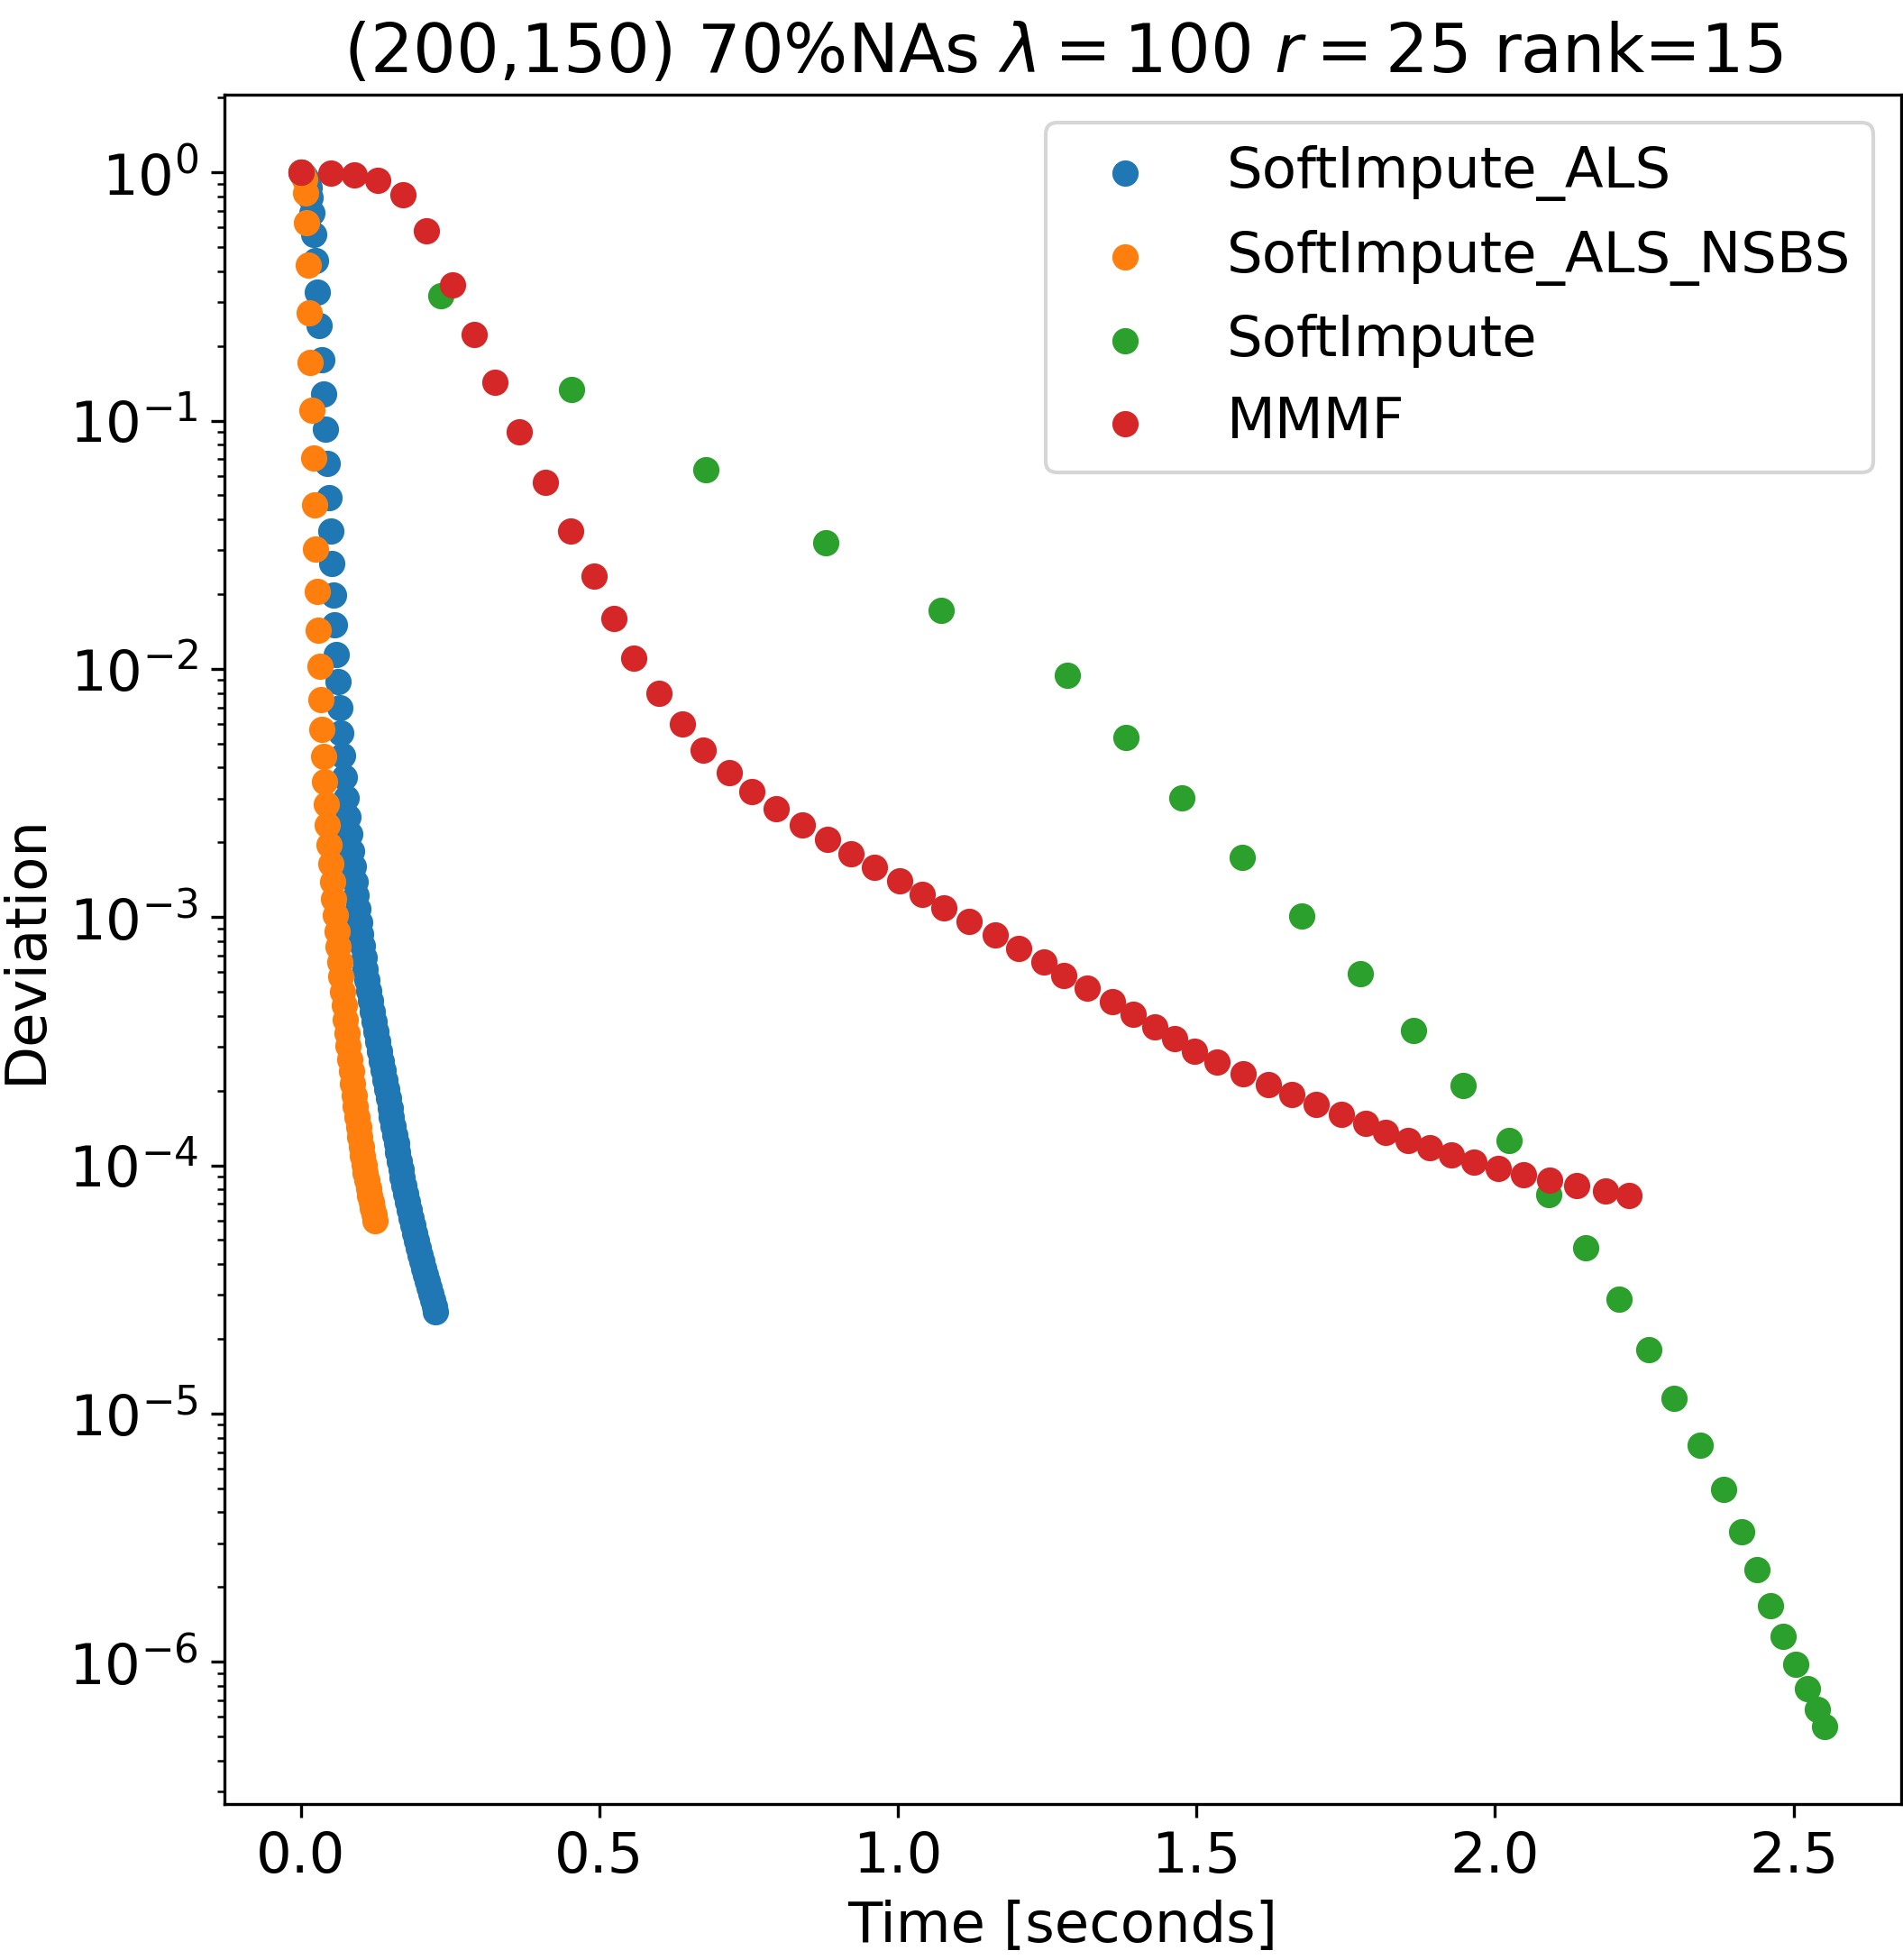
\includegraphics[scale=0.35]{timing_experiment_case1.png}              
	\end{minipage}}
	\subfigure[Case 2]{  
		\begin{minipage}{6.6cm}\centering   
			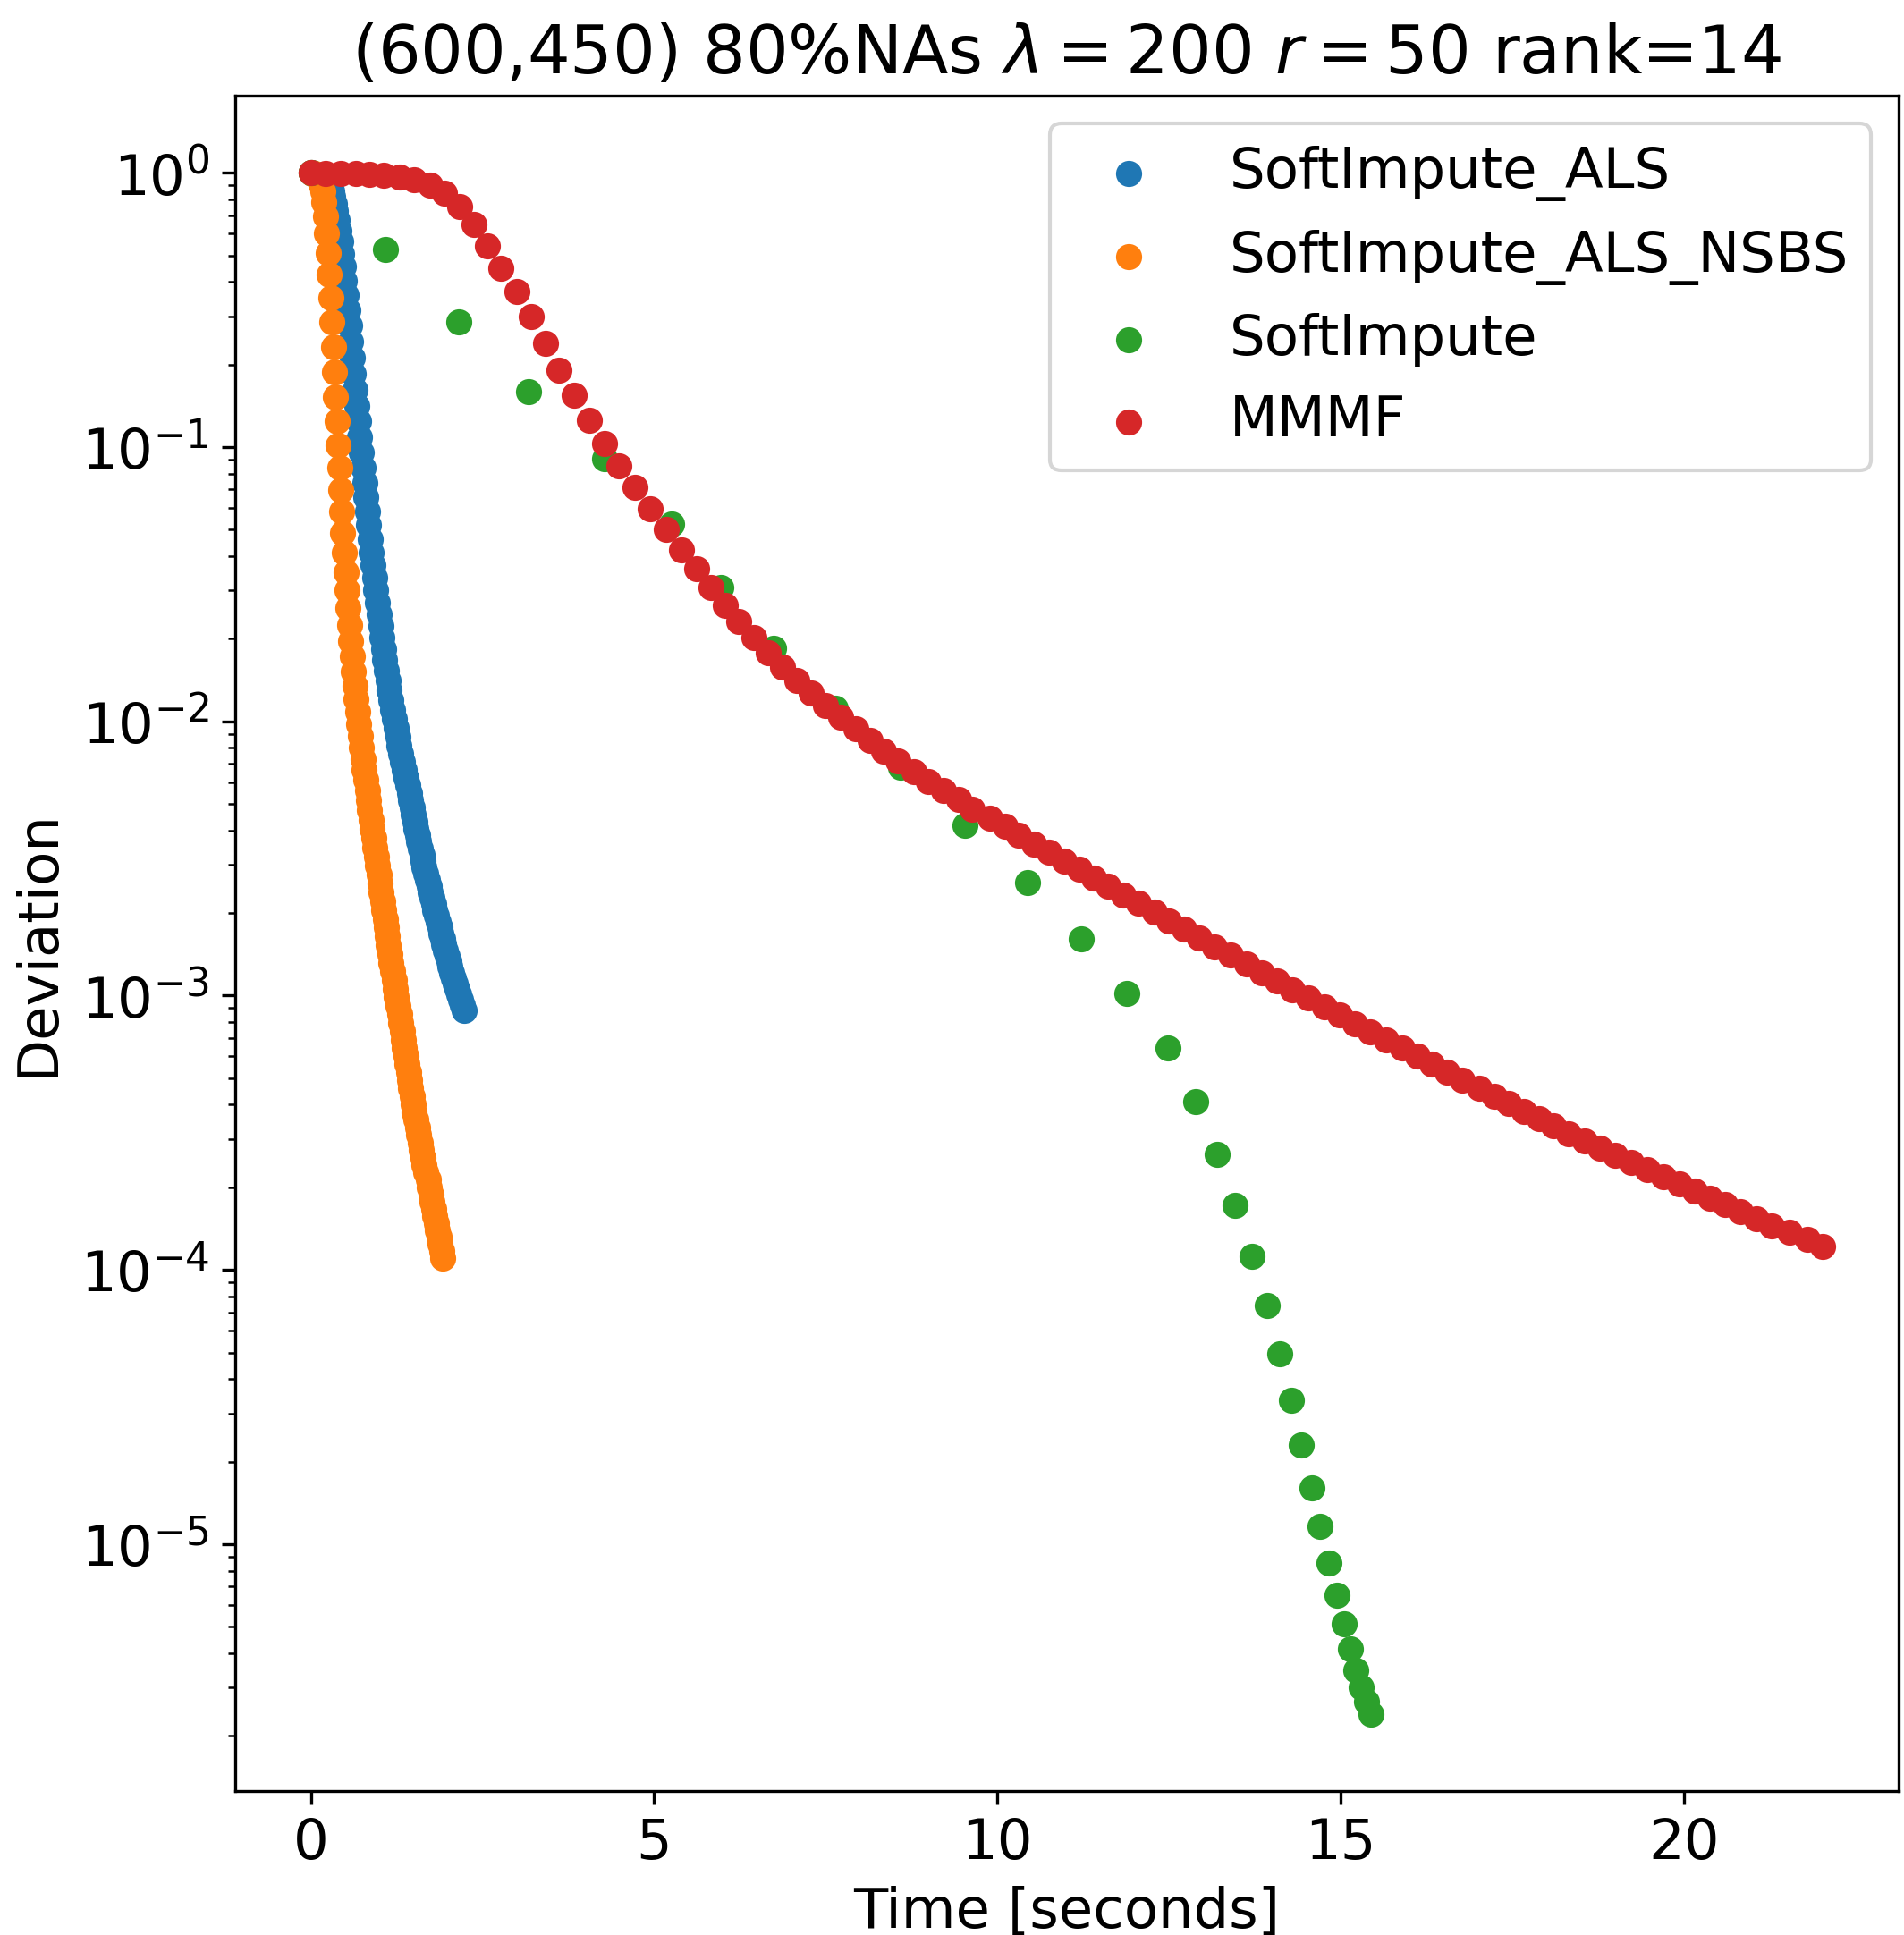
\includegraphics[scale=0.35]{timing_experiment_case2.png}        
	\end{minipage}}
	\subfigure[Case 3]{                   
	\begin{minipage}{6.6cm}\centering                                                         
		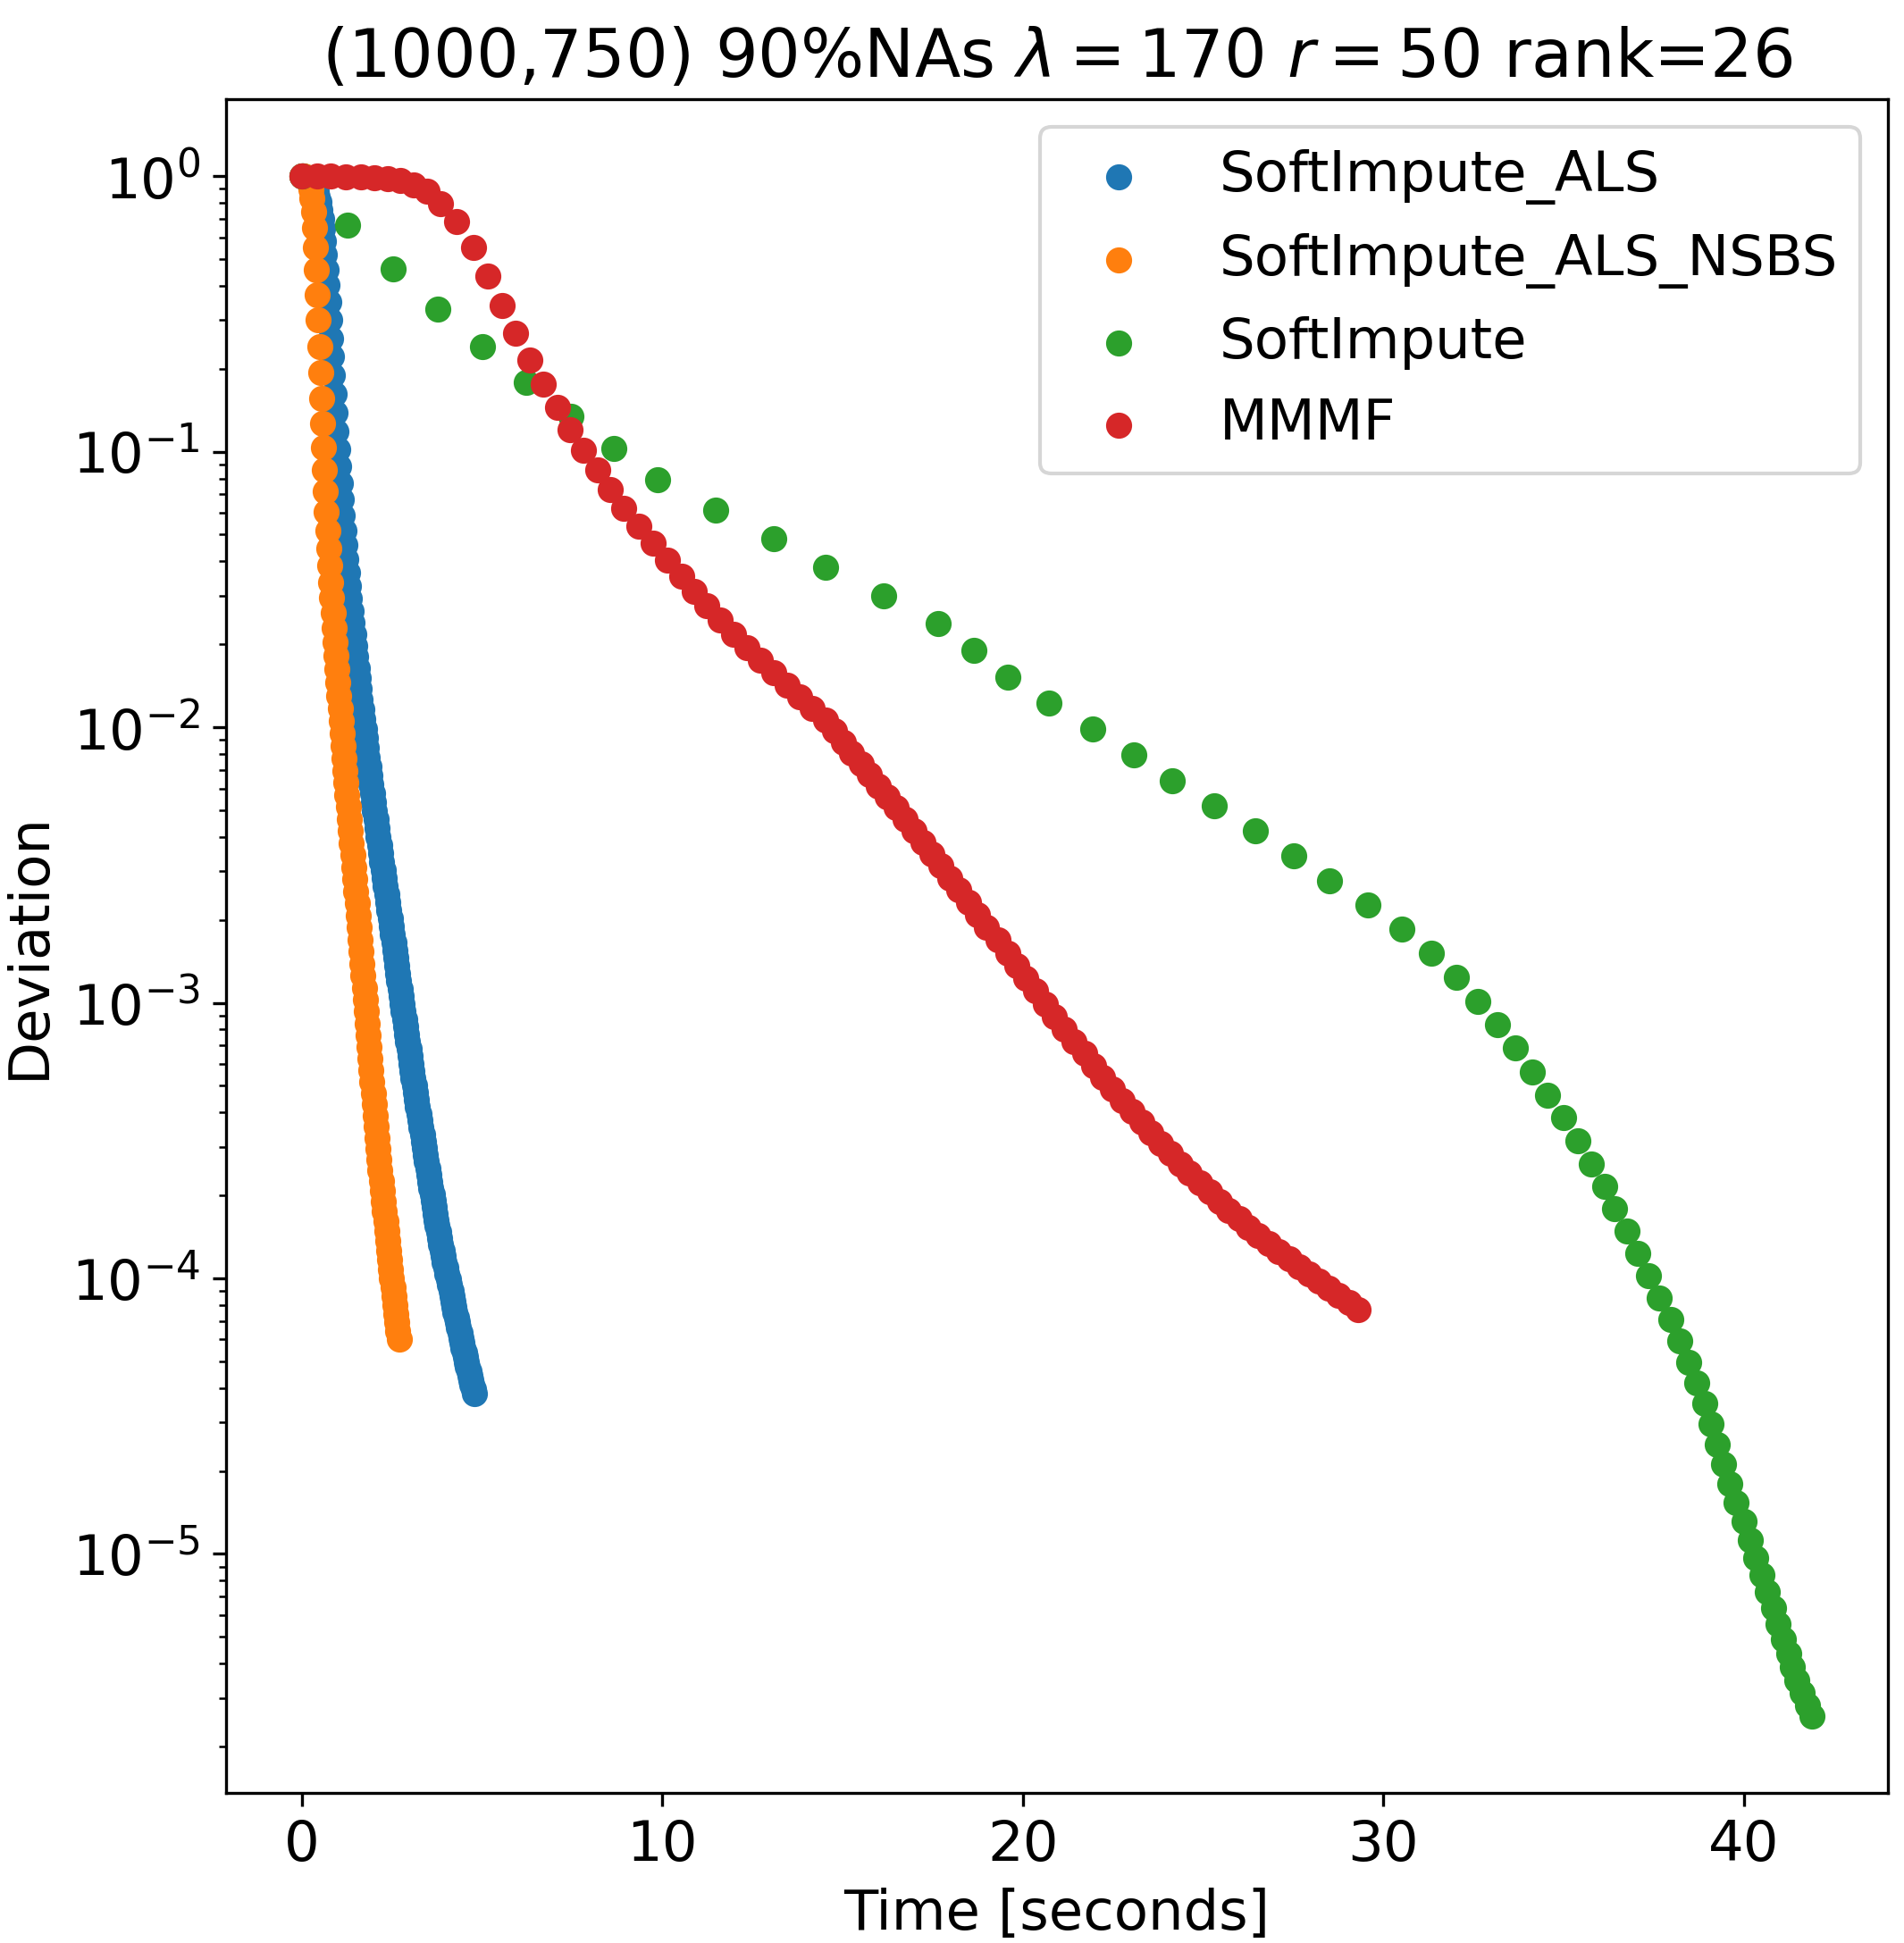
\includegraphics[scale=0.35]{timing_experiment_case3.png}              
\end{minipage}}
\subfigure[Case 4]{  
	\begin{minipage}{6.6cm}\centering   
		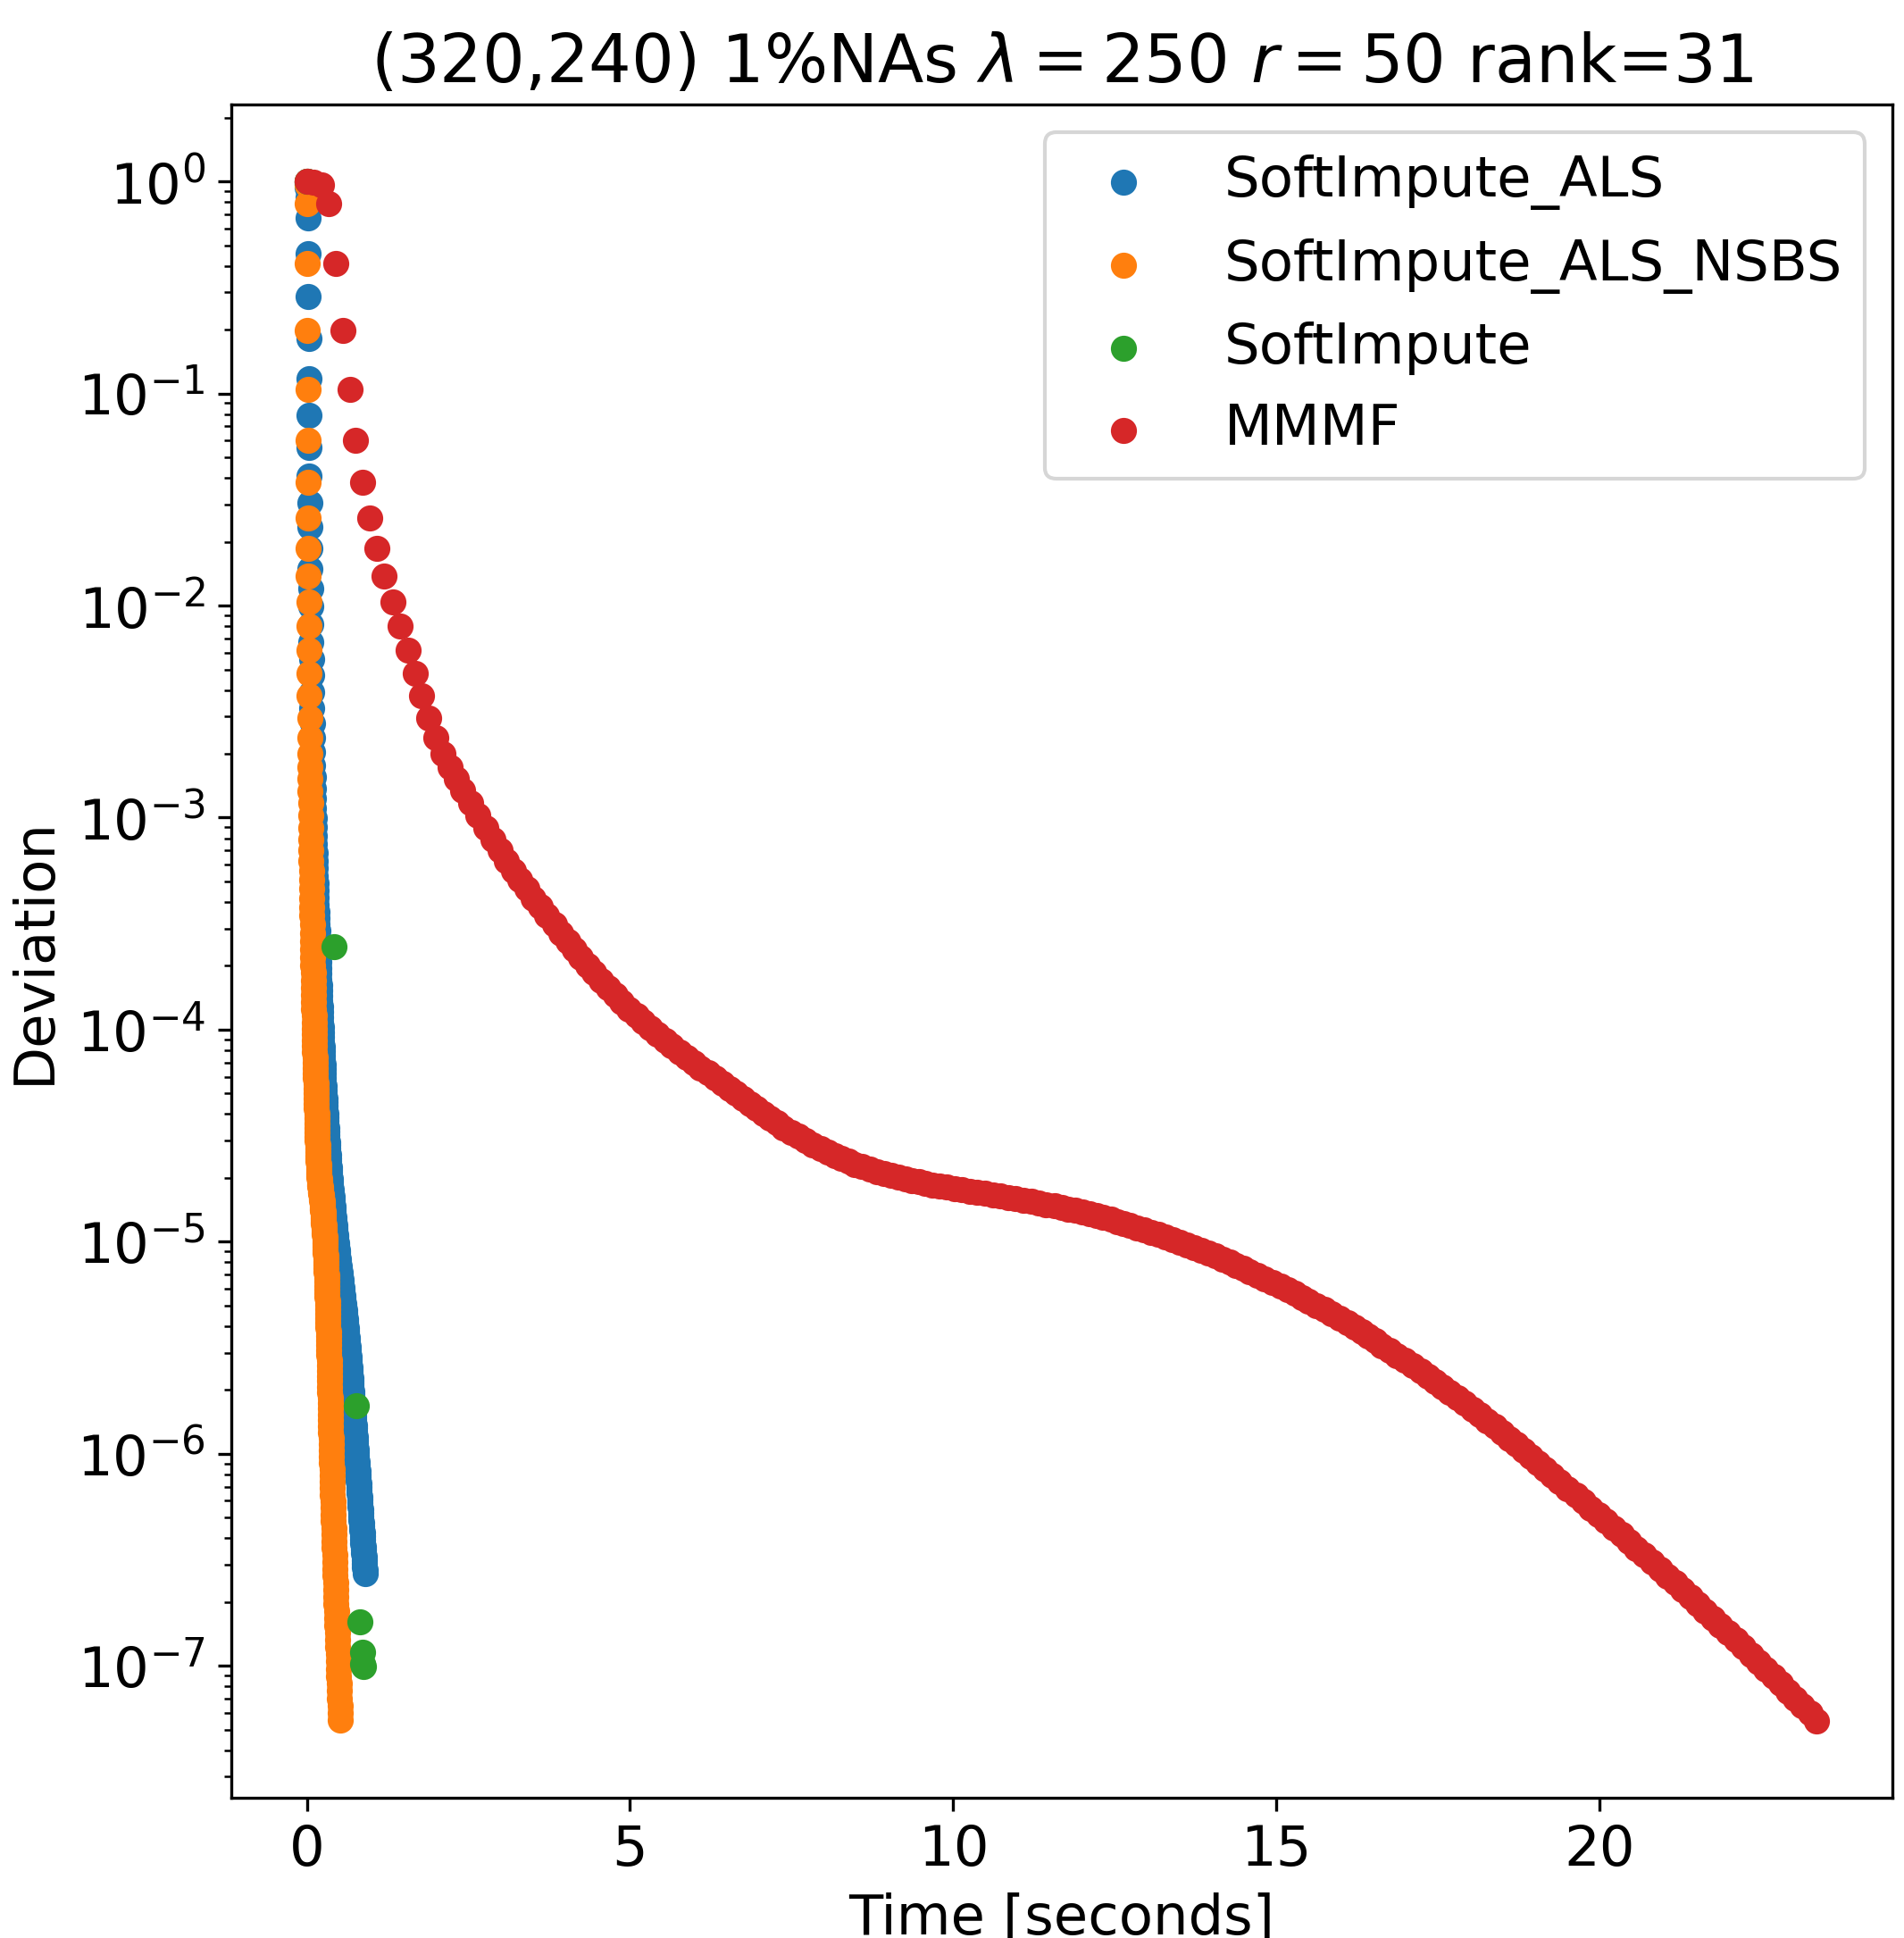
\includegraphics[scale=0.35]{timing_experiment_case4.png}       
\end{minipage}}
\caption{Four timing experiments. Each subfigure is labeled by the shape of $\boldsymbol{X}$, the proportion of missing values, the tuning parameter $\lambda$, the operating rank r for factorization, and estimated rank respectively. }
\label{fig:1}	                                                    
\end{figure}

	From Figure \ref{fig:1}, we can know that \textbf{SoftImpute-ALS},\textbf{SoftImpute-ALS-NSBS} have the fastest computation speed, while \textbf{MMMF} and \textbf{softImpute} are slower. The reasons are: (1) The cost of each iteration of \textbf{MMMF} is $O(r)$ times that of \textbf{SoftImpute-ALS}; (2) The cost of SVD of \textbf{softImpute} in the first several steps is much larger. The tails of the curves of \textbf{softImpute} also show that the cost of SVD will be much smaller due to the use of warm start using the previous solutions. Figure \ref{fig:1}d is the case that only 1\% entries are missing. In this case, \textbf{softImpute} performs pretty well that a good solution will be obtained by only few iterations. The interpretation for this phenomenon is that when the proportion of missing entries are very small, $P_{\Omega}(\boldsymbol{X})+P_{\Omega}^{\perp}(\boldsymbol{A}^k(\boldsymbol{B}^k)^T)$ will change very small, the SVD can directly obtain a good solution. In all experiments, we can find that \textbf{SoftImpute-ALS} and \textbf{SoftImpute-ALS-NSBS} have similar performance.

	Next, we will show that using \textbf{SoftImpute-ALS} as warm start of \textbf{softImpute} performs better than only using \textbf{SoftImpute-ALS}. To validate this claim, we simulate another experiment. The shape of $\boldsymbol{X}$ is (2000,1500) with true rank 120 and 50\% entries missing. We set the operating rank $r=50$. We run \textbf{SoftImpute-ALS} by 150 iterations at first, and then the current solution will be used as warm start of \textbf{SoftImpute-ALS}. \textbf{SoftImpute-ALS} will stop after 200 iterations. \textbf{SoftImpute-ALS} will stop after 350 iterations. Since we do not know the limiting objective or solutions, we set the minimal objective $f_{min}$ in the running process as the baseline, and then we define relative objective as $|f^k-f_{min}|/|f_{min}|$. 
	
	The following Figure \ref{fig:2} plots the result of relative objective to time, which shows the faster convergence rate of \textbf{softImpute} using warm start. Generally speaking, one iteration of \textbf{softImpute} can have more decline of current objective that that of \textbf{SoftImpute-ALS}, since SVD contains inner-loop alternating subspace methods similar to the explicit factorization in \textbf{SoftImpute-ALS}.
	
\begin{figure}[ht!]\centering
	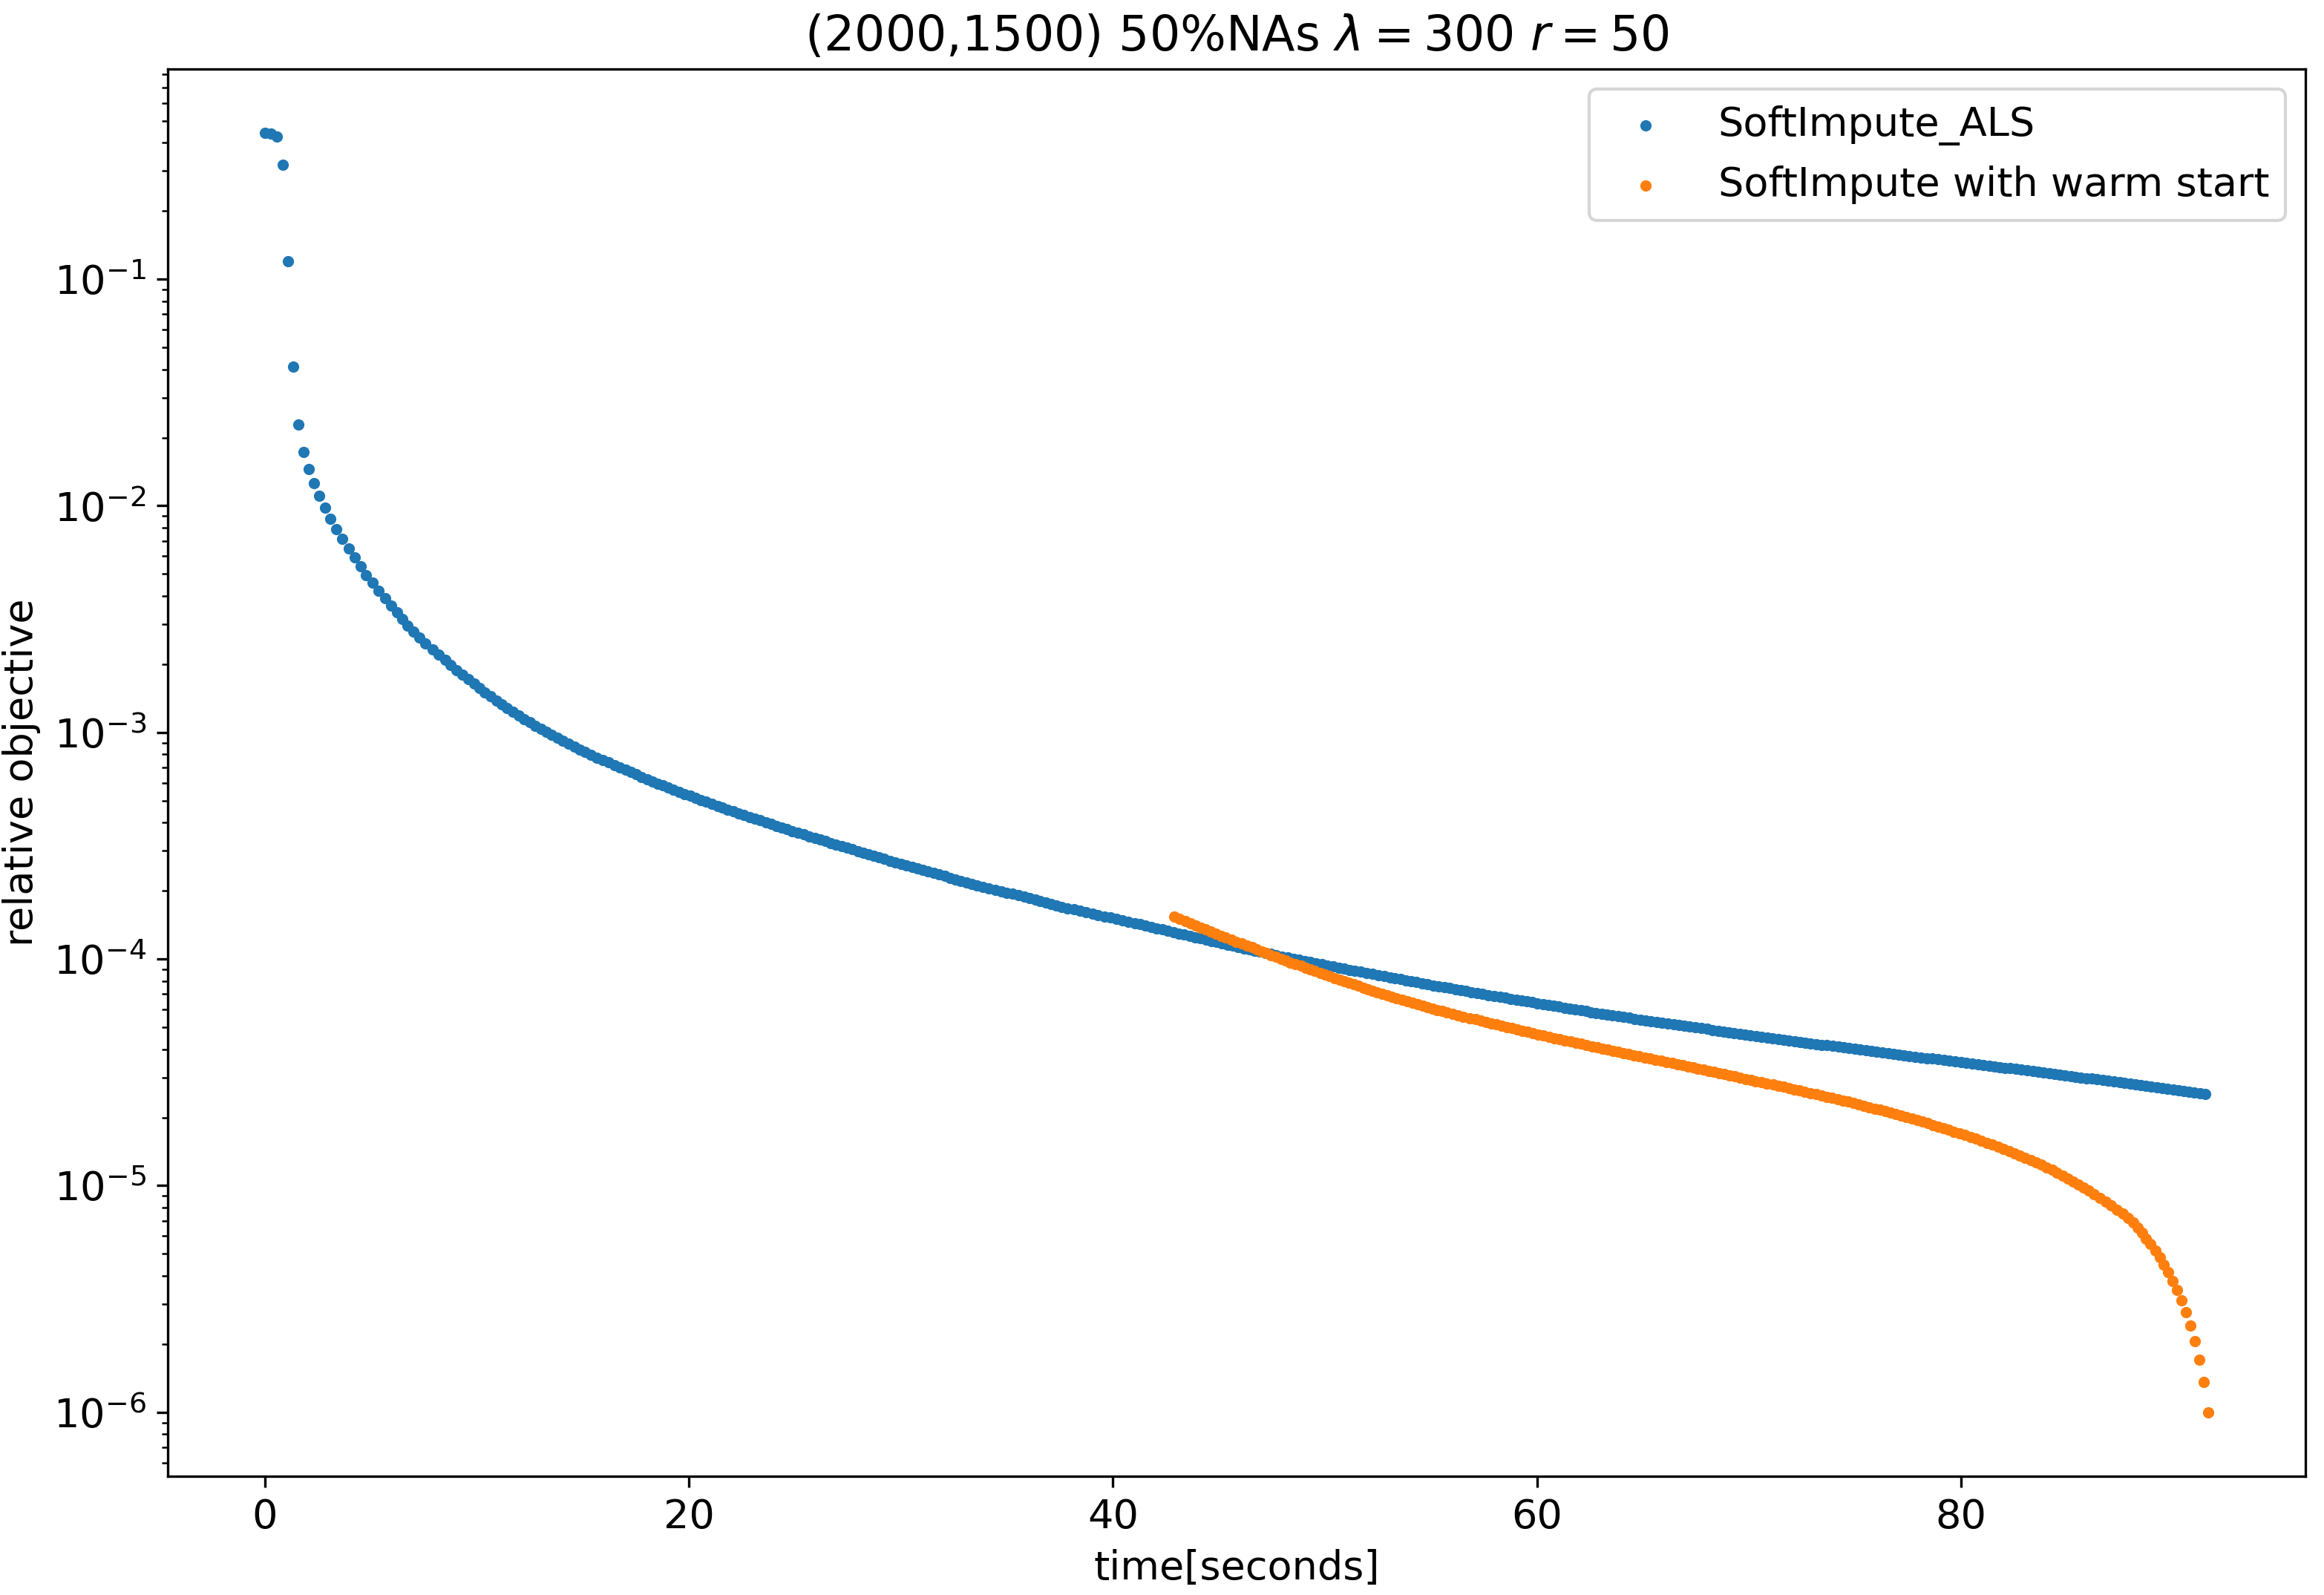
\includegraphics[scale=0.35]{warm_start.png}
	\caption{Warm start result. }
	\label{fig:2}	                                                    
\end{figure}
\subsection{Train and test error experiments}
	In the above subsection, we have compared the computational speed. In this subsection, we want to show the train and test errors of comparison algorithms. We still use the model mentioned in the above experiments. 
The SNR is defined as $SNR=\sqrt{\mathrm{var}(\boldsymbol{A}\boldsymbol{B}^T)/\mathrm{var}(\boldsymbol{E})}$. Therefore, when $\sigma=1$, we have $SNR=1$, and $SNR=10$ if $\sigma=0.1$.  The shape of $\boldsymbol{X}$ is (100,100) with true rank 15. We test two experiments, there are 60\% missing entries and $SNR=1$ in the first case, while the second case we set 50\% missing entries and $SNR=10$. We define train error as $\|P_{\Omega}(\boldsymbol{X}-\boldsymbol{X}_{est})\|_F^2/\|P_{\Omega}(\boldsymbol{X})\|_F^2$, where $\boldsymbol{X}_{est}$ is the obtained solution under specific tuning parameters. The test error is defined as $\|P_{\Omega}^{\perp}(\boldsymbol{A}\boldsymbol{B}^T-\boldsymbol{A}_{est}\boldsymbol{B}_{est}^T)\|_F^2/\|P_{\Omega}^{\perp}(\boldsymbol{A}\boldsymbol{B}^T)\|_F^2$. \textbf{SoftImpute-ALS} and \textbf{softImpute} are compared. For \textbf{softImpute-ALS}, there are two parameters $r$  and $\lambda$, while only $\lambda$ for \textbf{softImpute}. The results are shown as Figure \ref{fig:3}, Table \ref{table: table 1}, and  Figure \ref{fig:4}. For \textbf{softImpute}, we also calculate the error after post-processing \citep[][Sec. 7]{mazumder2010spectral}.

\begin{figure}[ht!]\centering                                                          
\subfigure[Train and test error and estimated rank of  \textbf{softImpute-ALS} when SNR=1.]{                   
	\begin{minipage}{14cm}\centering                                                         
			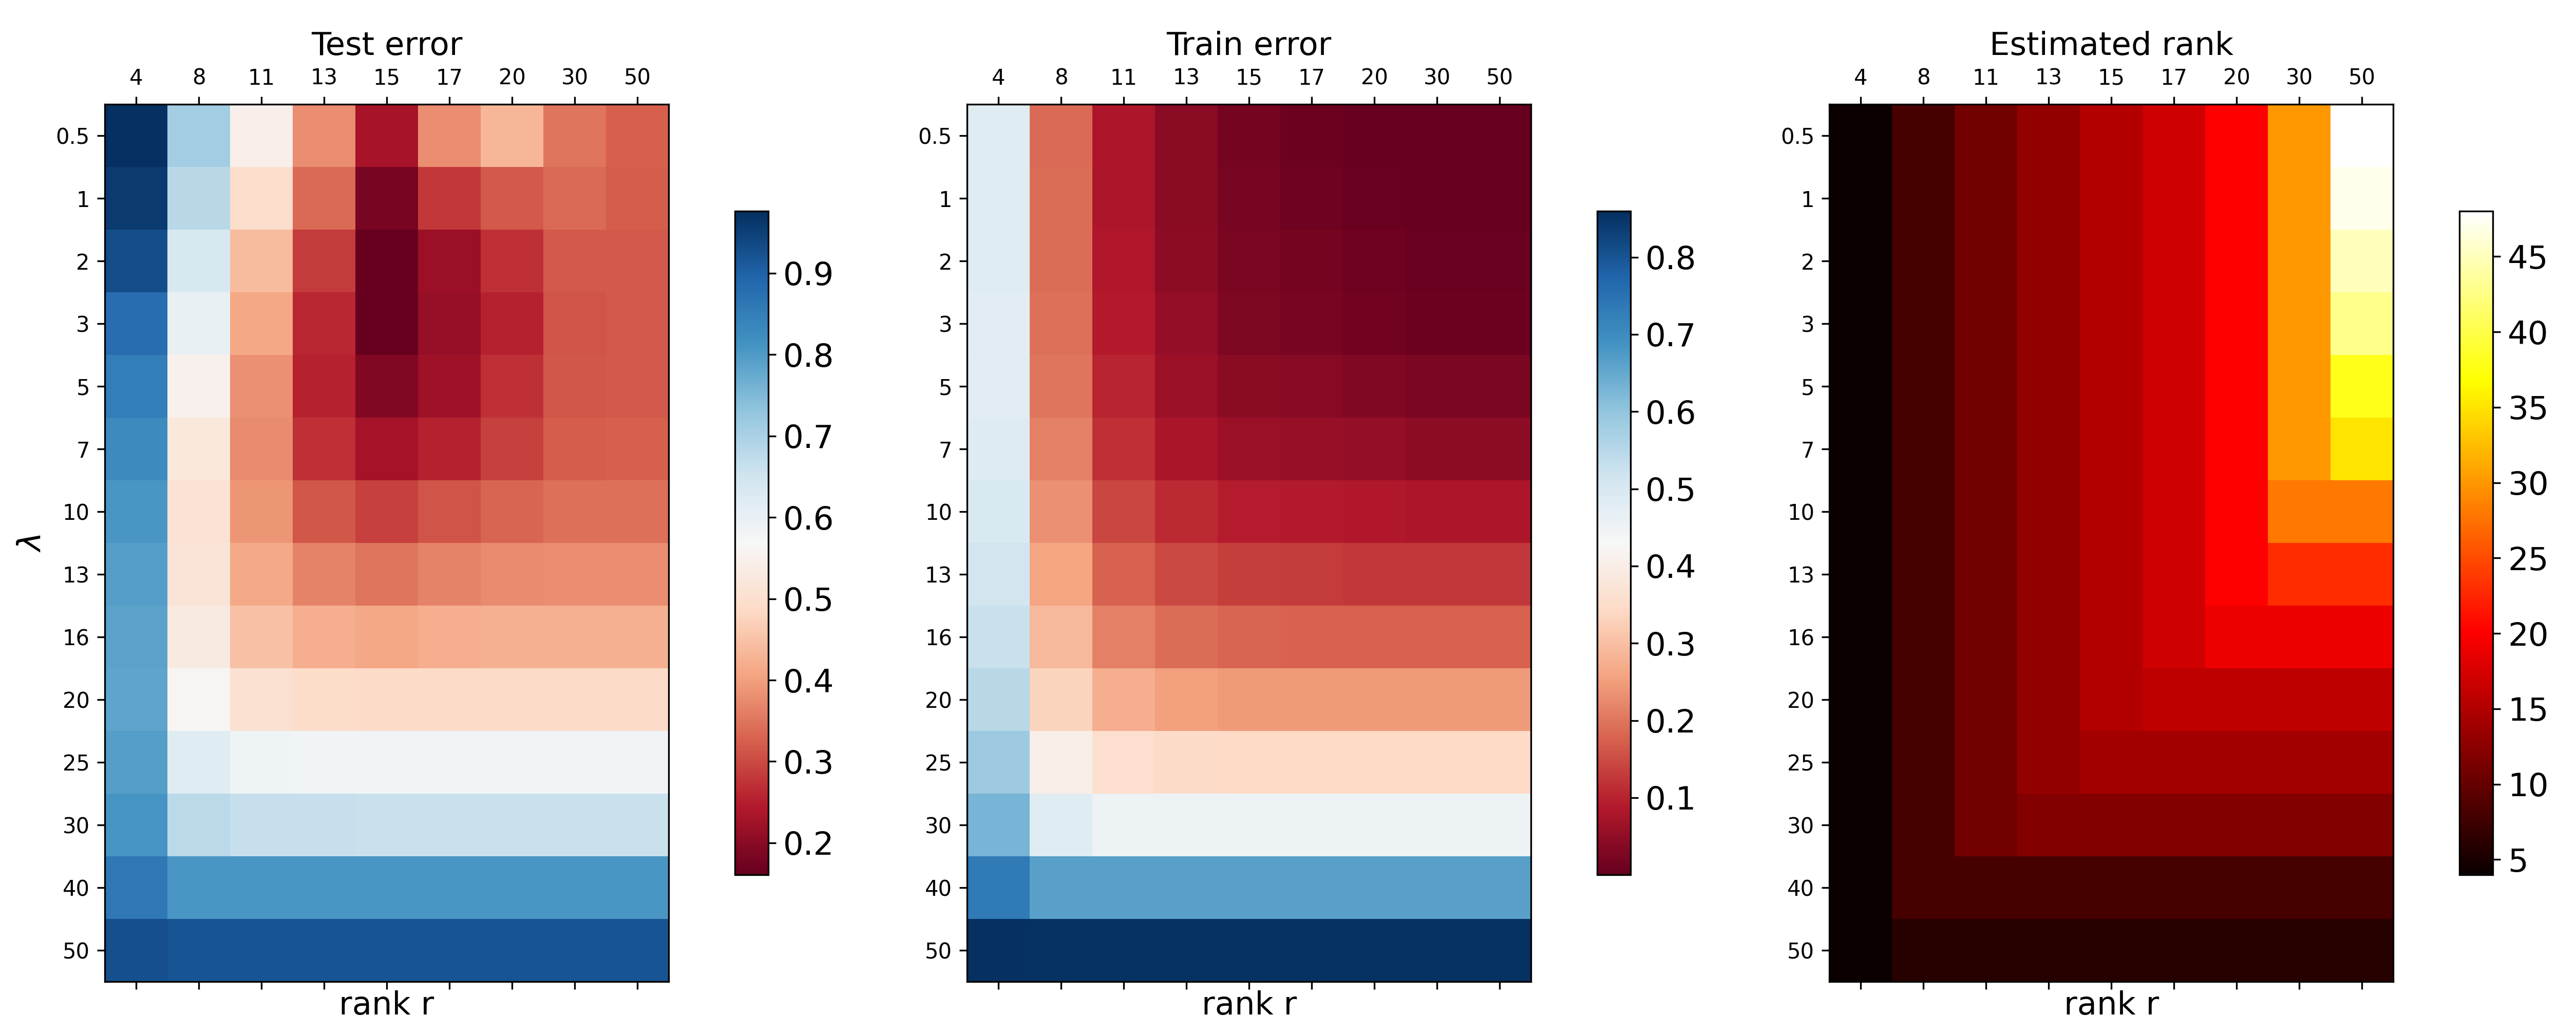
\includegraphics[scale=0.35]{test_train_error_ALS.png}              
	\end{minipage}}
	\subfigure[Train and test error and estimated rank of  \textbf{softImpute-SVD} when SNR=1.]{                   
		\begin{minipage}{14cm}\centering                                                         
			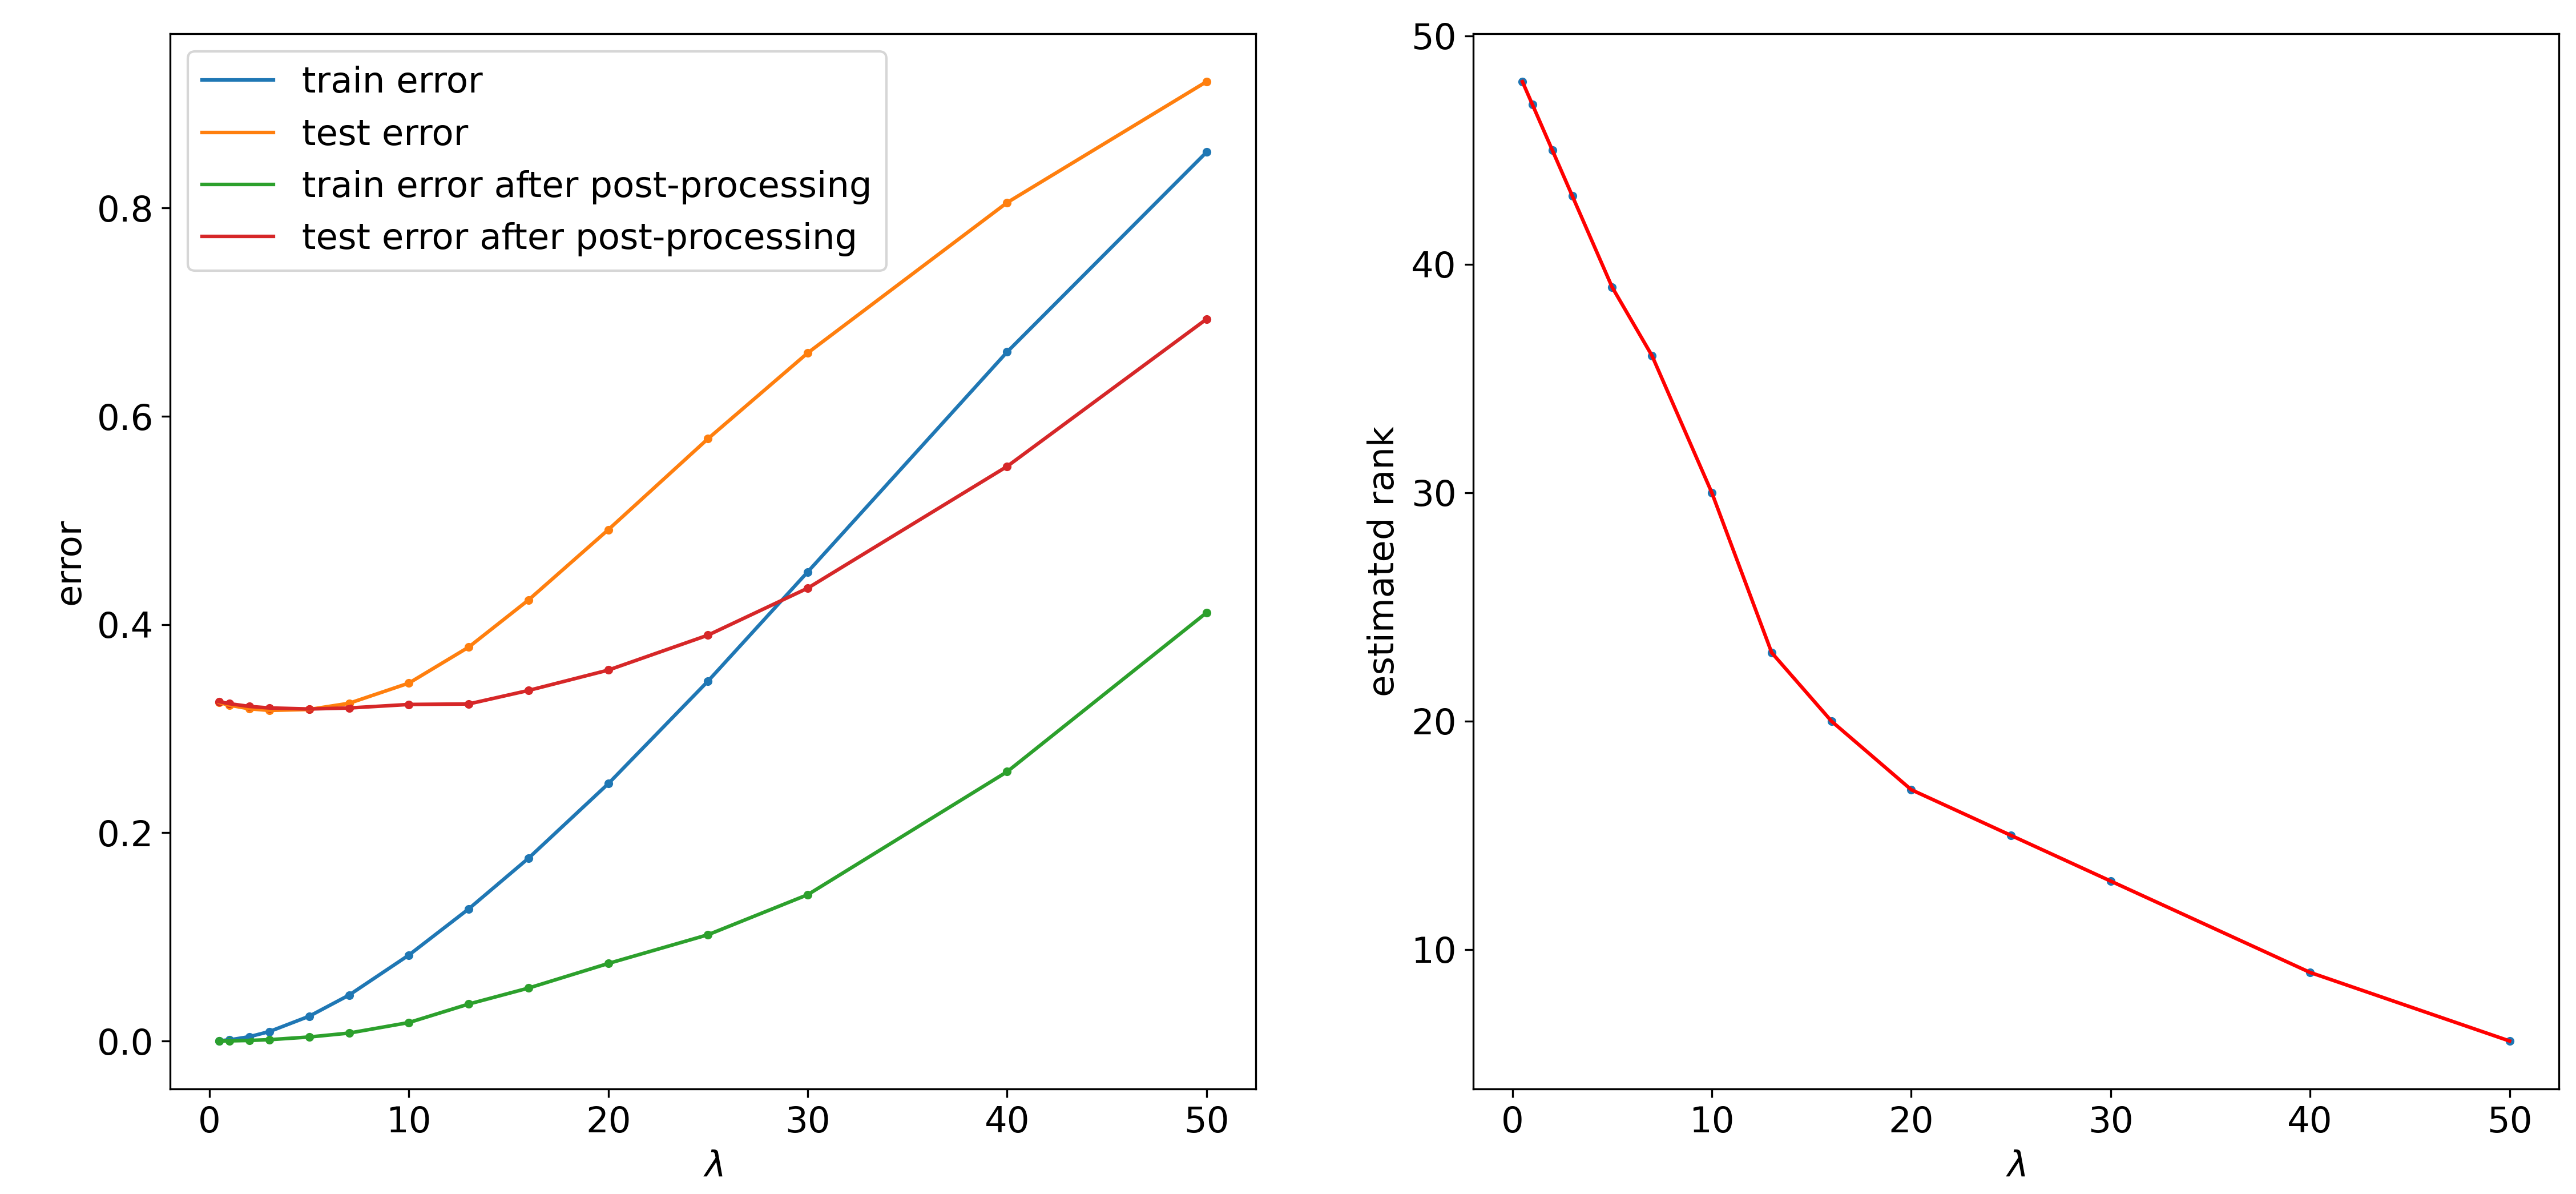
\includegraphics[scale=0.32]{test_train_error_SVD.png}              
	\end{minipage}}
	\caption{The first case with 60\% missing entries and $SNR=1$.}
	\label{fig:3}	                                                    
\end{figure}

\begin{table}[t!]
	\caption{Minimal test error of \textbf{softImpute-ALS} and  \textbf{softImpute-SVD}.} 
	\centering 
	\begin{tabular}{c c c c c} 
		\hline\hline 
		\multirow{2}{*}{ } & \multicolumn{2}{c}{\textbf{softImpute-ALS}} & \multicolumn{2}{c}{\textbf{softImpute}} \\ \cline{2-5}
		&SNR=1&SNR=10&SNR=1&SNR=10 \\ \hline
		minimal test error&0.1609 &0.0010&0.3189&0.0149 \\ \hline

		
	\end{tabular}
	
\label{table: table 1} 
\end{table}


\begin{figure}[ht!]\centering                                                          
	\subfigure[Train and test error and estimated rank of  \textbf{softImpute-ALS} when SNR=10.]{                   
		\begin{minipage}{14cm}\centering                                                         
			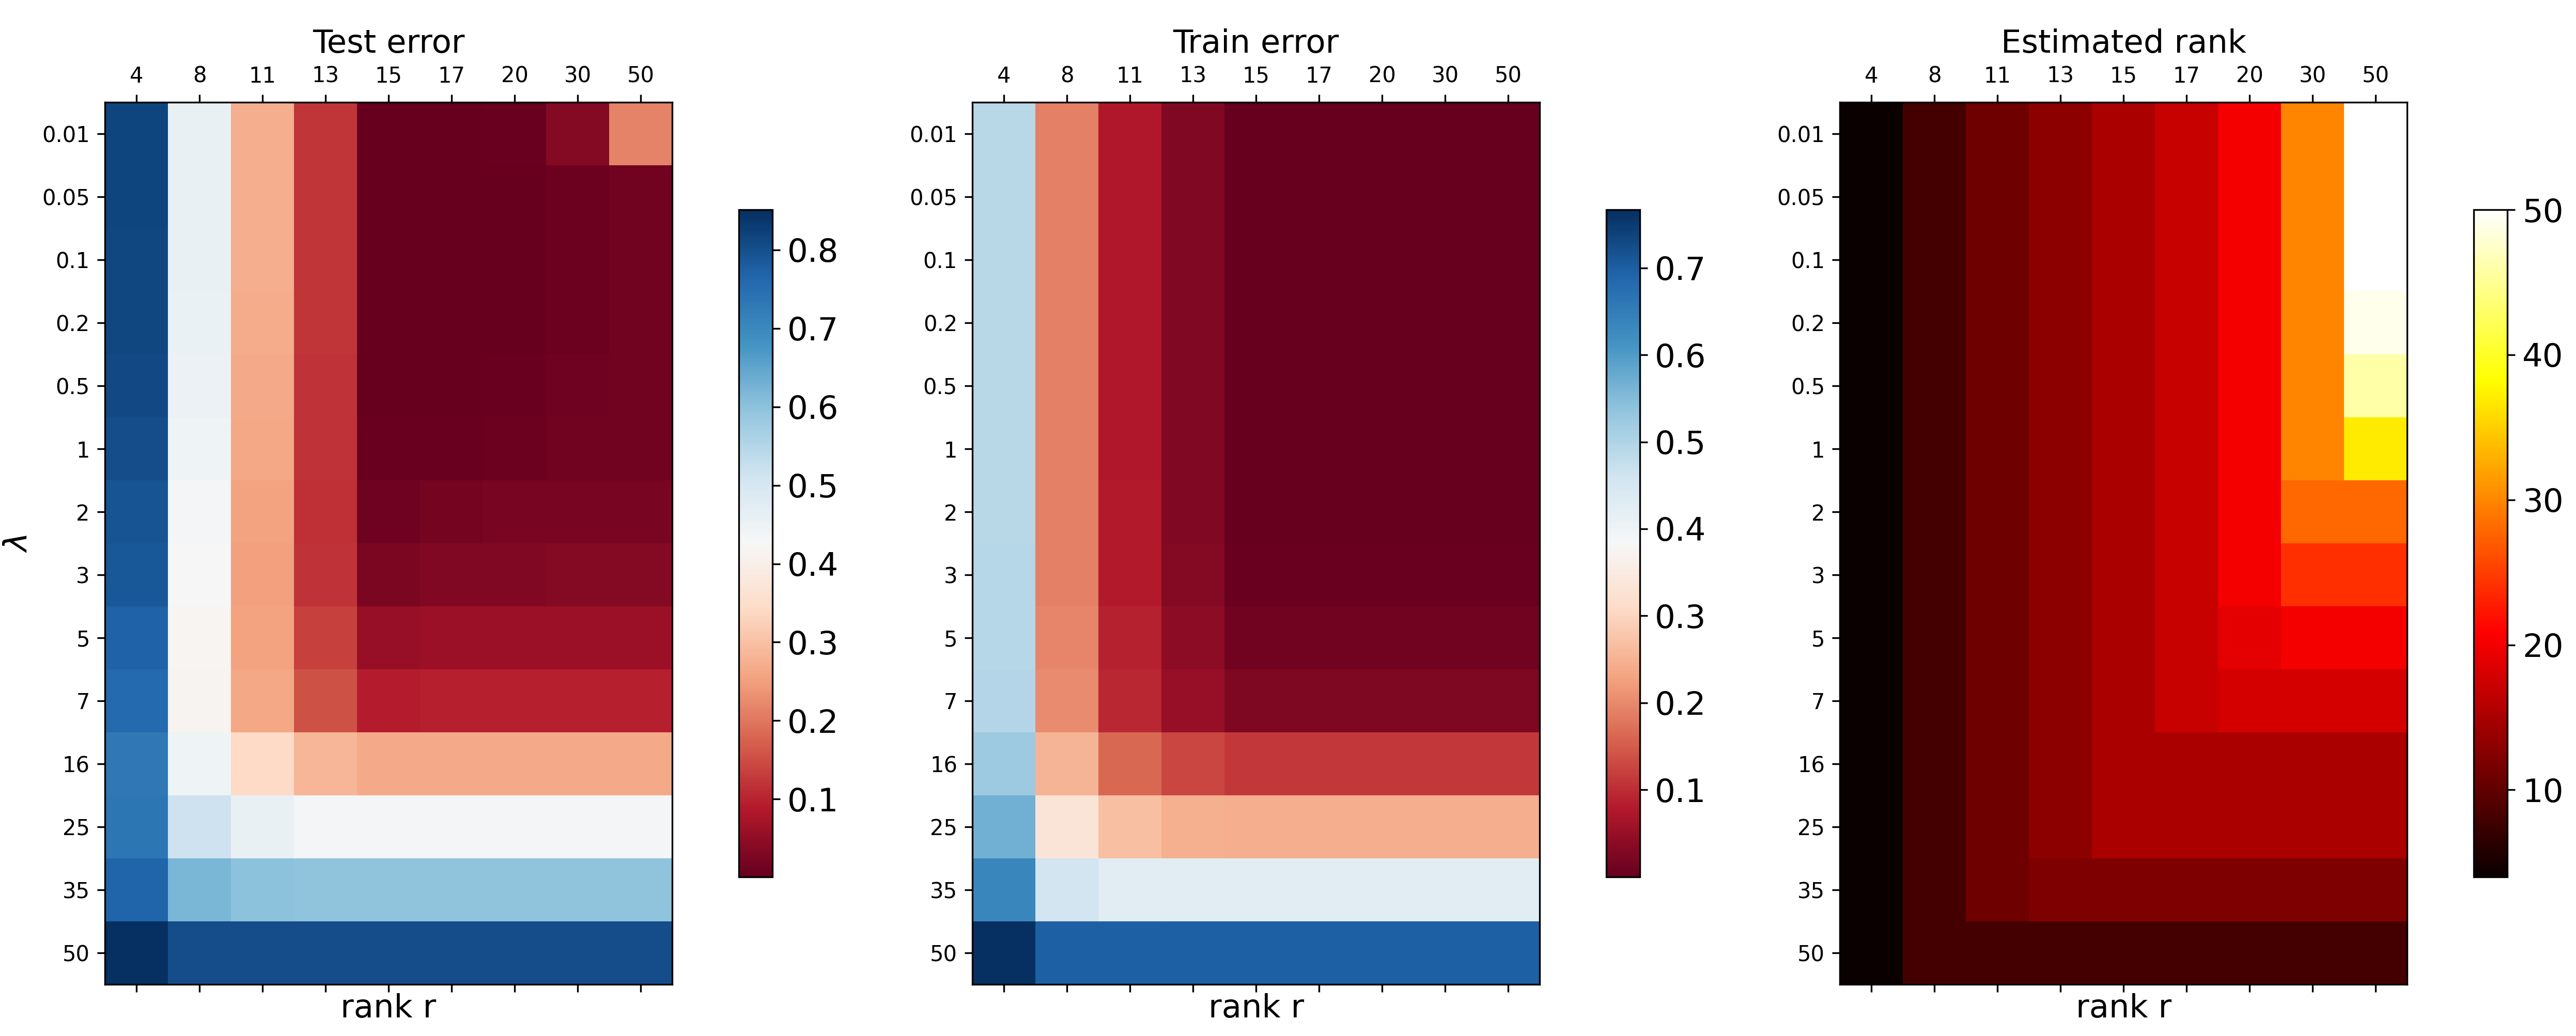
\includegraphics[scale=0.35]{test_train_error_ALS_case2.png}              
	\end{minipage}}
	\subfigure[Train and test error and estimated rank of  \textbf{softImpute-SVD} when SNR=10.]{                   
		\begin{minipage}{14cm}\centering                                                         
			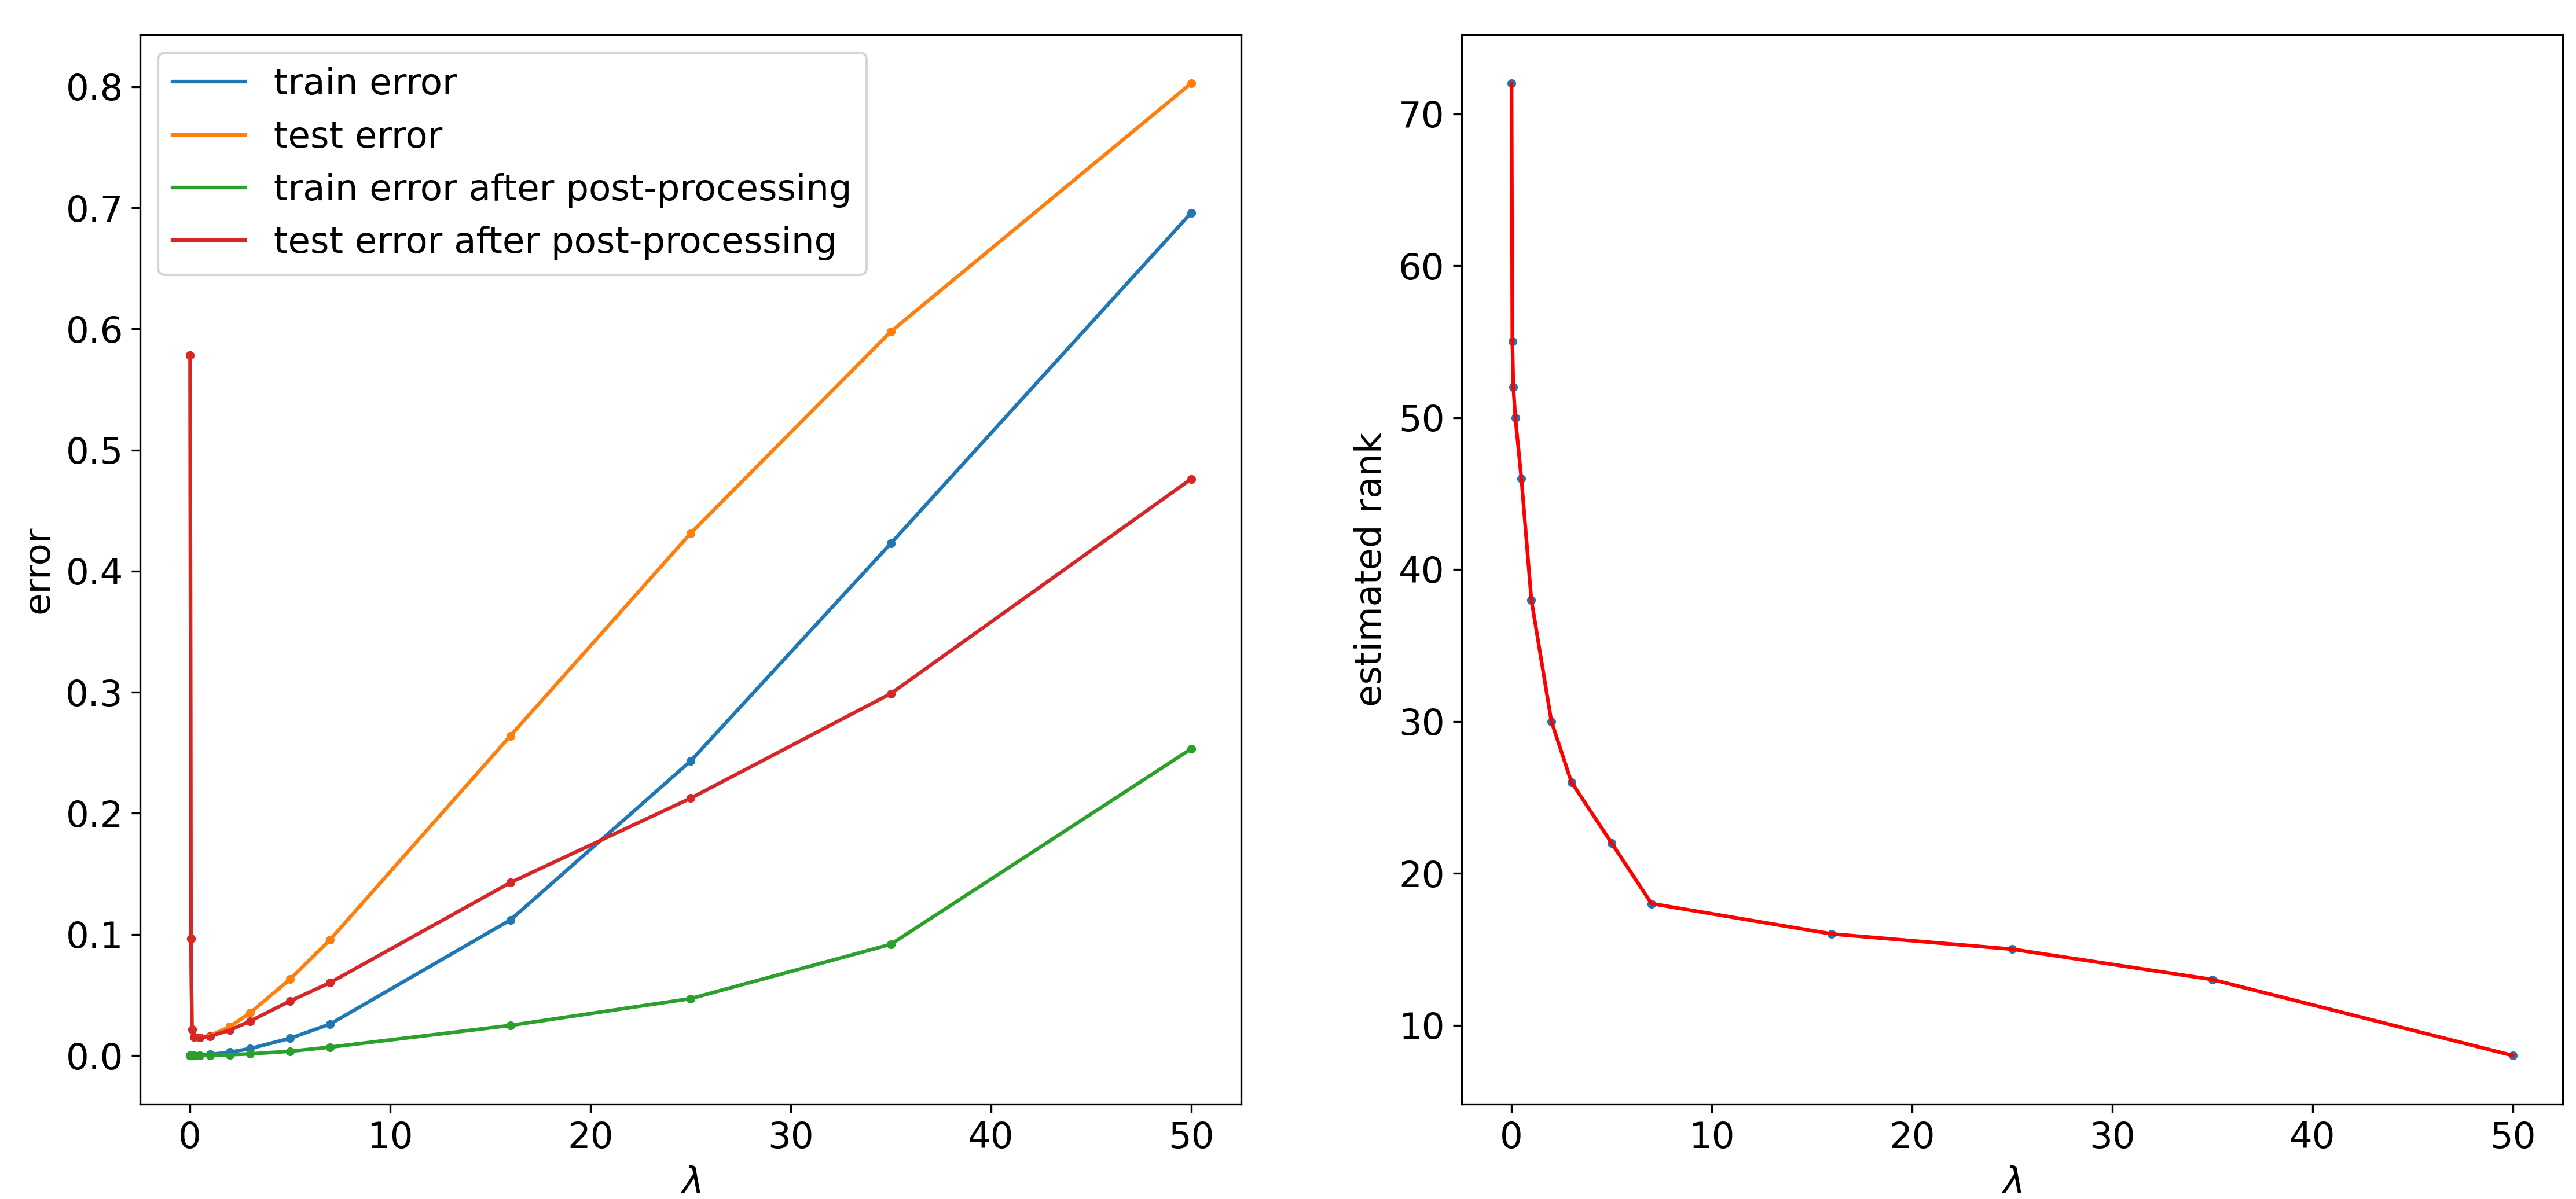
\includegraphics[scale=0.32]{test_train_error_SVD_case2.png}              
	\end{minipage}}
	\caption{The second case with 50\% missing entries and $SNR=10$. }
	\label{fig:4}	                                                    
\end{figure}

The results suggest that \textbf{softImpute-ALS} is better than \textbf{softImpute} in terms of train error and test error. The reason may be the fact that \textbf{softImpute-ALS} contains another tuning parameter $r$, which can provide some prior information about our model. Indeed, we can observe from the test error colormap in Figure \ref{fig:3}a that test error reach minimum when $r=15$, which is the true rank. Table \ref{table: table 1} illustrates that the additional regularization of $r$ leads to much lower test error both in SNR=10 and SNR=1. Though \textbf{softImpute-ALS} works better, the selection of two-family tuning parameters is more difficult in practice.
 
\section{Conclusion}
This paper propose \textbf{softImpute-ALS} for matrix completion problem. This method combines \textbf{softImpute} and \textbf{MMMF}, which has faster computation speed. We validated this point by simulation experiments. Moreover, we found that using  \textbf{softImpute-ALS} as warm start for \textbf{softImpute} can achieve the better performance than separate ones. We also calculated the train error and test error of  \textbf{softImpute-ALS} and \textbf{softImpute}. The results show that \textbf{softImpute-ALS} has lower minimal test error due to the additional regularization of the operating rank $r$.


\bibliographystyle{chicago}

\bibliography{ref.bib}

\end{document}